%%%%%%%%%%%%%%%%%%%%%%%%%%%%%%%%%%%%%%%%%%%%%%%%%%%%%%%%%%%%%%%%%%%%%%%%%%%%%%%%%%%%%%%%%%%%%%%%%%%%%%%%%%%%%%%%%%%%%%%
%
%  Filename   : preamble.tex
%
%  Description: Preamble file to :
%               a. specify related packages
%               b. set margins, commands, etc.
%
%  Note       : Edit the margin settings for your own printer
%                  You may add your own commands, environments (it is assumed that you know what you're doing.)
%
%%%%%%%%%%%%%%%%%%%%%%%%%%%%%%%%%%%%%%%%%%%%%%%%%%%%%%%%%%%%%%%%%%%%%%%%%%%%%%%%%%%%%%%%%%%%%%%%%%%%%%%%%%%%%%%%%%%%%%%

%\documentclass[12pt,titlepage,onepage, letterpaper]{article}

\documentclass[12pt,titlepage,onepage,letterpaper]{report}


%
%-- specify related packages
%

%
% \usepackage[utf8x]{inputenc}
%

\usepackage{pdfpages}

\usepackage{apacite}           %-- APA style citation 
                               %-- refer to http://www.ctan.org/tex-archive/biblio/bibtex/contrib/apacite/

%
%  \usepackage{ucs}
%


\usepackage{amsmath}           %-- American Math Society packages
\usepackage{amsfonts}
\usepackage{amssymb}
\usepackage{booktabs}
\usepackage{array}             %-- column types for tables
\newcolumntype{L}[1]{>{\raggedright\arraybackslash}p{#1}}   %-- ragged-right paragraph column (narrow table cells)

\usepackage{tikz}              %-- diagrams drawn in LaTeX (used for the pipeline figure, no participant images)
\usetikzlibrary{positioning,arrows.meta}
\usepackage[chapter]{algorithm} %-- algorithm floats, numbered within chapters
\usepackage{algpseudocode}     %-- pseudocode inside algorithm floats

\usepackage{graphicx}          %-- graphicx package needed for including figures in JPG or PNG format
 
%
%\usepackage{graphics}          %-- graphics related package (this was commented out) use when image is in EPS format
%

\usepackage{verbatim}          %-- this package allows you to have multiple lines of comments by
                               %-- example:
                               %   \begin{comment}
                               %        ...your text here...
                               %   \end{comment}  

\usepackage{color}             %-- allows use of color with text
                               %-- example:  \textcolor{red}{This is the colored text in red.}

\usepackage{url}  %-- allows use of URLs example: \url{https:\ccs1.dlsu.edu.ph}


%
%-- set margins,  you may need to edit this for your own printer
%
\topmargin 0.0in
\oddsidemargin 0.0in
\evensidemargin 0.0in

\voffset 0.0in
\hoffset 0.5625in

\textwidth 5.75in
\textheight 8.5in


\parskip 1em
\parindent 0.25in

\bibliographystyle{apacite}            %-- use APA citation scheme

\hyphenation{ana-lysis know-ledge}     %-- LaTeX may not hyphenate correctly some words you use in your document
                                       %-- use \hyphenation to instruct LaTeX how to do it correctly, example above

\newcommand{\degree}{^{\circ}}         %-- use \newcommand to create your own "commands"
                                       %-- \newcommand works like the #define you learned in your COMPRO1 class

\newcommand{\etal}{et al.}

%-- Visible marker for decisions still pending (proponent or adviser). Remove all uses before submission.
\newcommand{\pending}[1]{\textcolor{red}{\textbf{[PENDING: #1]}}}
%-- Visible question for the adviser to read in the PDF. Remove all uses before submission.
\newcommand{\askadviser}[1]{\textcolor{red}{\textbf{[#1]}}}


%\newcommand{\sinag}{\emph{Sinag}}
%\newcommand{\sinagtwo}{\emph{Sinag2}}

\newcommand{\figref}[1]{Figure \ref{#1}}
\newcommand{\appref}[1]{Appendix \ref{#1}}

%-- \newcommand{\Section}[1]{\section{#1}\setcounter{figure}{0}\setcounter{table}{0}}

%\newcommand{\shade}{\multicolumn{1}{|>{\columncolor[gray]{0.25}}c|}{}}
%\newcommand{\tableheader}[1]{\rowcolor{black}\color{white}{#1}}
%\newcommand{\cell}[2]{\multicolumn{1}{#1}{#2}}
%\newcommand{\definition}[2]{\textbf{\textit{#1}} --- #2}
%\newcommand{\itembit}[1]{\item \textbf{\textit{#1}}}
%\newcommand{\sgdef}[2]{\parbox[t][][t]{1.75in}{\textbf{#1}} \> \parbox[t][][t]{4.0in}{#2}\\\\}

%\newenvironment{sinagglossary}{\begin{flushleft}
%\begin{tabbing}
%\hspace{1.75in}\=\\}{\end{tabbing}\end{flushleft}}

\newcommand{\thestitle}[1]{{\Large \textsc{#1}}}


%---
%  \renewcommand{\thefigure}{\thesection.\arabic{figure}}
%  \renewcommand{\thetable}{\thesection.\arabic{table}}
%  \renewcommand{\contentsname}{Table of Contents}




                %-- includes LaTeX source file for the preamble 

\begin{comment}
Description: 
This is the main file for the LaTeX thesis proposal document template. The template is intended for use by students under the Department of Software Technology. 

It is assumed that you can learn how to use LaTeX on your own. Please check/read the following online LaTeX book:
http://en.wikibooks.org/wiki/LaTeX
     
Author: Florante R. Salvador

Contributors: 
1.  Karlo Campos (former faculty member)
2.  Briane Paul V. Samson 
   
Notes: 
Please email the DST Graduate School Coordinator for feedback and suggestions

History/Updates:
March 12, 2009:
    -- created version 1.0 for release to CSC701M (Methods of Research) students
May 30, 2009   
    -- updated Title page and Abstract for undergrad ST students
Feb 27, 2015 (version 2)
    -- changed class to report, created a figures folder, removed unnecessary packages, added new comments  based on Ethel Ong's slides
Feb 24, 2018 (version 3)
    -- Reorganized the chapters, i.e., Chapter 3 is now Theoretical Framework and Chapter 4 is now Research Methodology.
    -- Included the Research Ethics documents as Appendix A.
June 15, 2022 (version 4)
    -- Updated the title page
    -- Revised text for figures and references
October 23, 2025 (version 5)
    -- Updated the title page by adding other degree programs
    -- Added abstract_fil for the thesis abstract in Filipino
\end{comment}

\graphicspath{{figures/}}  %-- figures is the name of the folder containing images JPG or PN

\begin{document}

%%%%%%%%%%%%%%%%%%%%%%%%%%%%%%%%%%%%%%%%%%%%%%%%%%%%%%%%%%%%%%%%%%%%%%%%%%%%%%%%%%%%%%%%%%%%%%%%%%%%%%
%
%   Filename    : title_page.tex 
%
%   Description : This file will contain your Title Page.
%                 
%%%%%%%%%%%%%%%%%%%%%%%%%%%%%%%%%%%%%%%%%%%%%%%%%%%%%%%%%%%%%%%%%%%%%%%%%%%%%%%%%%%%%%%%%%%%%%%%%%%%%%

\begin{titlepage}
\centering


%-- **EDIT** the following line to indicate your thesis title. Try to keep it within 20 words for brevity, and focus on highlighting the intended contribution of your work.
\thestitle{Position-Based versus Content-Based Frame Selection for Detecting Student Engagement in Video-Based Learning}

\vspace{1.5cm}

A Thesis Proposal\\
%A Thesis\\

\vspace{0.5cm}

presented to\\

\vspace{0.5cm}

the Department of Software Technology\\
College of Computer Studies\\
De La Salle University

\vspace{1cm}

In partial fulfillment\\
of the requirements for the degree of\\

\vspace{0.5cm}

Bachelor of Science in Computer Science and \\
Master of Science in Computer Science

%Master of Science in Computer Science

%Master of Science in Data Science

%Doctor of Philosophy in Computer Science

%Doctor of Philosophy in Data Science

%Doctor of Philosophy in Artificial Intelligence

\vspace{1.75cm}

by \\


%% EDIT the following line to indicate the complete names of all your group members arranged in alphabetical order 
\vspace{1cm}

SITYAR, Lester Anthony Jr.  \\

\vspace{1.75cm}
%-- **EDIT** the following line to indicate your adviser's name 
Judith AZCARRAGA \\
Adviser

\vspace{1.75cm}
\today
\end{titlepage}
              %-- includes LaTeX source file for the Title Page 
                                  %-- your job: **EDIT THIS FILE ** to indicate your own title, name, and thesis adviser's name


\begin{comment}
This file will contain your abstract in English.
Template rules: 150 to 250 words, one paragraph, no citations or quotes. Moves: motivation,
problem, contribution, methodology. The template skips results at the proposal stage, but the
adviser asked (11 Nov 2026) for the preliminary study's results to be included.
\end{comment}

\begin{abstract}
Detecting student engagement automatically from webcam video could help instructors in online learning notice when students disengage. Video-based engagement classifiers often process only a few frames of each clip, yet the rule that chooses these frames has rarely been studied on its own. A preliminary study on the EngageNet dataset compared a fixed Start-Middle-End rule with selecting three, five, or seven frames at peaks of facial-landmark velocity. All four classifiers had their highest mean macro F1 with three velocity-peak frames, the best being a Support Vector Machine at 0.70. The gain over Start-Middle-End, however, was significant only for a Random Forest, by up to 4.79 accuracy points, and the design could not separate how frames are chosen from how many are kept or from chance. This study will determine whether content-based frame selection improves the classification of observer-rated engagement over position-based and random selection with the same number of frames. Positional, random, velocity-peak, and Bayesian changepoint selection will each keep three, five, or seven frames of every EngageNet clip, and four classifiers will separate Highly-Engaged clips from all others using MediaPipe face and pose features. The study will also test whether representing the order and change of the selected frames improves on averaging them. Conditions will be compared clip by clip with McNemar tests, corrected for multiple comparisons and repeated over five seeds or random draws, and with equivalence tests, which check whether two configurations differ by less than two accuracy points, a margin set before any results are seen.

\begin{flushleft}
\begin{tabular}{lp{4.25in}}
\hspace{-0.5em}\textbf{Keywords:}\hspace{0.25em} & Student engagement detection, frame selection, temporal sampling, affective computing, video classification, E-learning \\
\end{tabular}
\end{flushleft}
\end{abstract}
                %-- this is the Abstract page in English
                                  %-- your job: **EDIT THIS FILE** to indicate your own abstract

\pagenumbering{roman}             %-- this will number pages as i, ii, iii, etc...
\setcounter{page}{2}

\tableofcontents                  %-- this command is used to generate the Table of Contents


\newpage
\listoffigures                    %-- this command is used to generate List of Figures

\newpage                       
\listoftables                     %-- this command is used to generate List of Tables

\newpage

\pagenumbering{arabic}            %-- this will number pages as 1, 2, 3, etc...
\setcounter{page}{1}              


%%%%%%%%%%%%%%%%%%%%%%%%%%%%%%%%%%%%%%%%%%%%%%%%%%%%%%%%%%%%%%%%%%%%%%%%%%%%%%%%%%%%%%%%%%%%%%%%%%%%%%
%
%   Filename    : chapter_1.tex
%
%   Description : Introduction. The scope is narrowed here in response to the OCE panel's comment
%                 that the scope was too broad.
%
%%%%%%%%%%%%%%%%%%%%%%%%%%%%%%%%%%%%%%%%%%%%%%%%%%%%%%%%%%%%%%%%%%%%%%%%%%%%%%%%%%%%%%%%%%%%%%%%%%%%%%

\chapter{Introduction}
\label{sec:intro}

This chapter introduces the study. Section~\ref{sec:overview} describes its background and states the research problem. Section~\ref{sec:objectives} states the objectives, Section~\ref{sec:scopelimitations} the scope and limitations, and Section~\ref{sec:significance} the significance of the research.


%%
%% --- 1.1 Background of the Study --- %%
%%

\section{Background of the Study}
\label{sec:overview}

Student engagement refers to a student's involvement in a learning activity, and it has behavioral, emotional, and cognitive dimensions \cite{fredricks2004}. Engagement is not fixed. It responds to features of the classroom, such as the task and the support a teacher gives \cite{fredricks2004}, which is one reason to measure it. Engagement has traditionally been measured through self-reports, teacher ratings, and observation. Automated measurement offers a further option: models infer engagement from behavioral and physiological signals, such as facial expressions and eye movements, at a finer time scale than questionnaires allow \cite{dmello2017}. Detecting learners' affective states and engagement from such signals is an established line of work in affective computing \cite{dmello2015}.

This study concerns video-based learning, in which students watch lecture videos or attend classes in front of a computer. In the Philippines, the Commission on Higher Education issued guidelines in 2020 for flexible learning in higher education institutions, which include online delivery \cite{ched2020}. In video-based learning, the webcam is a readily available sensor, cheaper and less intrusive than physiological devices \cite{abedi2021}. Datasets such as DAiSEE \cite{gupta2016} and EngageNet \cite{singh2023} record students watching learning videos through a webcam and label each short clip with the level of engagement that human observers judged it to show. In EngageNet, three observers rated each ten-second clip on four levels, taking gaze, head pose, and facial expression into account \cite{singh2023}.

Research on these datasets has concentrated on features and network architectures. On DAiSEE, for example, reported four-level accuracy has risen from 57.9\% to 67.5\% (Section~\ref{sec:rw-models}). Less attention has been paid to which frames of a clip reach the classifier. A ten-second clip contains well over a hundred frames, and most of the approaches reviewed in Section~\ref{sec:rw-frameuse} either use every frame or keep a fixed subsample. When only a few frames are kept, which ones are kept may matter: observers' clip-level judgments can be predicted from individual frames \cite{whitehill2014}, and in video understanding more broadly, the rule that selects frames measurably affects results \cite{korbar2019,brkic2025}. Two studies have compared frame selection rules for students' states. \citeA{resurreccion2024} compared a fixed rule with changepoint-based selection, each keeping three frames, for classifying academic emotions in DAiSEE. The preliminary study of this proposal \cite{sityar2026icce} compared Start-Middle-End (SME) sampling, which keeps the first, middle, and last frames, with the selection of three, five, or seven frames at peaks of facial-landmark velocity in EngageNet. All four classifiers tested had their highest mean macro F1 under three-frame velocity-peak selection, but the improvement over SME was statistically significant for only one of them.

Neither comparison can show why one rule did better than another. In both, the position-based rule was tested at only three frames, so the effect of how frames are chosen cannot be separated from the effect of how many are kept. Neither included random selection, so neither can show whether choosing frames by their content does better than choosing them arbitrarily. The problem this study addresses is therefore the following: it is not known whether selecting frames by their content improves the classification of observer-rated engagement over selecting them by position, or over selecting them at random, when the same number of frames is kept. The first two research questions are: \emph{How does content-based frame selection compare with position-based and random selection in classifying observer-rated student engagement at equal frame budgets?} and \emph{How does this comparison vary with the frame budget and the classifier?} A related choice is how the selected frames are then combined into one input. Many classifiers average them, which discards their order, and whether order and change add information is unsettled, particularly when only a few frames are kept (Section~\ref{sec:rw-temporal}). The third research question is therefore: \emph{What are the effects of representing the order and change of the selected frames on engagement classification, compared with averaging them?}


%%
%% --- 1.2 Research Objectives --- %%
%%

\section{Research Objectives}
\label{sec:objectives}

\subsection{General Objective}

The general objective of this study is to determine whether selecting the frames of a video clip by their content improves the classification of observer-rated student engagement compared with selecting them by their position in the clip.

\subsection{Specific Objectives}

The specific objectives of this research are as follows:
\begin{enumerate}
   \item To extract facial and upper-body pose features from the EngageNet video clips;
   \item To characterize content-based, position-based, and random frame selection techniques by their effect on engagement classification;
   \item To evaluate techniques for representing the temporal aspect of the selected frames, such as their order and how they change, when the frames are combined into a single input for engagement detection;
   \item To implement and evaluate various machine learning classifiers for detecting student engagement from the selected frames; and
   \item To determine the best-performing combination of frame selection technique, number of frames, frame combination technique, and classifier.
\end{enumerate}


%%
%% --- 1.3 Scope and Limitations --- %%
%%

\section{Scope and Limitations of the Research}
\label{sec:scopelimitations}

\textbf{Data and participants.} The study uses EngageNet \cite{singh2023} only, with its official subject-independent partition: 91 training, 11 validation, and 26 test participants, counted by subject identifier (Section~\ref{sec:data}). The participants were 127 adults, 83 male and 44 female, aged 18 to 37, recorded by webcam while watching instructional videos in settings such as computer laboratories, dormitory rooms, and open spaces \cite{singh2023}. The study uses pre-existing data only. No new data will be collected. Only the video is used. Audio, interaction data, and participants' answers to comprehension questions are not, because the observers' ratings were based on visible behavior. EngageNet's documentation describes its participants only by sex and age range, and the dataset was not collected for Filipino learners or in Philippine classrooms. The results may therefore not carry over to Filipino students or to other datasets, whose settings and labels differ (Section~\ref{sec:rw-datasets}).

\textbf{Data preparation (Objectives 1 and 3).} Every clip is turned into classifier input in the same way in every condition. Clips labeled Subject Not Present are removed, and the remaining labels are reduced to the binary task described below. Within each clip, a frame is valid when a face is detected and the detected face and body are consistent with each other (Section~\ref{sec:features}). A selection rule, described in the next paragraph, chooses up to $k$ of the valid frames. For each selected frame, features are extracted with MediaPipe \cite{lugaresi2019}: 478 facial landmarks and 52 blendshape scores from its Face Landmarker, and eight upper-body keypoints from its Pose Landmarker, 1,518 values in all. MediaPipe is kept from the preliminary study, and the same tool provides both the landmark positions that the two content-based rules need and the features the classifiers receive. The same features are used in every condition, so that only the frames selected and the way they are combined change the input. Other feature sets are not compared. In particular, the study does not use the action units of OpenFace 2.0 \cite{baltrusaitis2018}, on which the EngageNet baselines were built \cite{singh2023}. Blendshapes have not been shown to work better than action units, and whether the findings hold with action units is not tested (Section~\ref{sec:indicators}). The selected frames of a clip are then combined into one input (Section~\ref{sec:temporal}). Three of the classifiers, a Multi-Layer Perceptron (MLP), a Support Vector Machine (SVM), and a Random Forest, receive a single vector, formed in four ways. The first is the mean of the frames, which carries no temporal information. The other three are temporal representations: the frames concatenated in order, the mean together with how much each feature changes between consecutive frames, and the mean together with how similar every pair of frames is. The fourth classifier, a Long Short-Term Memory network (LSTM), reads the frames in order and combines its outputs either by averaging them or by attention. These representations use only the selected frames. Neither the timing of the frames within the clip nor information from frames that were not selected is used, so that the selection rules remain comparable. Features are standardized with statistics from the training split before changes and similarities are computed, and the SVM and Random Forest receive standardized inputs. SMOTE oversampling \cite{chawla2002} then balances the training data in every condition (Section~\ref{sec:training}). The validation and test clips are never oversampled. Other representations, including those learned by other sequence models, are not compared.

\textbf{Frame selection (Objective 2).} Five selection rules are studied: two position-based rules (SME and positional), random selection as a control, and two content-based rules ($k$-Changepoint and $k$-BOCPD). Positional, random, $k$-Changepoint, and $k$-BOCPD selection are each applied at three, five, and seven frames, and SME at three frames only, which gives thirteen selection conditions. The frame budgets of three, five, and seven frames extend the preliminary study. Comparing SME with positional selection at three frames tests whether including the first and last frames of a clip matters. All conditions use the same clips (Section~\ref{sec:commonset}). Dense sampling of every frame, and learning which of all the frames to use, as attention over every frame does, are outside the scope. The two content-based rules define content differently (Section~\ref{sec:changepoint}). The $k$-Changepoint rule, kept from the preliminary study, selects the frames at which the face moves fastest, a minimal case of changepoint detection. The $k$-BOCPD rule uses Bayesian online changepoint detection (BOCPD) \cite{adams2007} to select the frames at which the face settles into a new position or expression. Comparing the two tests whether fast movement or lasting change marks the more useful frames. Other changepoint methods, such as PELT \cite{killick2012}, are not tested. Like BOCPD, PELT divides the signal into segments of stable behavior, and the study compares these two kinds of content, not every changepoint method.

\textbf{Task and classifiers (Objective 4).} The four engagement levels are reduced to one binary task: Highly-Engaged clips against all others. This task is retained from the preliminary study (Section~\ref{sec:binarization}). The full training split is close to balanced under it (3,740 Highly-Engaged against 4,139 other clips). The four-level task is outside the scope. So is the separate detection of Not-Engaged clips, although these are arguably the most important to detect in practice. They stay in the negative class for three reasons: a single task keeps the study focused on frame selection, the preliminary results that motivate the design exist only for this task, and a second task would double the 254 planned comparisons (Section~\ref{sec:evaluation}). How often Not-Engaged clips are mistaken for Highly-Engaged ones is still reported for every condition (Section~\ref{sec:metrics}). The four classifiers keep the same settings in every condition, and these settings are not tuned, so a difference between two conditions can be attributed to the frames selected and the way they are combined rather than to tuning. They are evaluated with macro F1, accuracy, and the Matthews correlation coefficient (Section~\ref{sec:measures}) on the subject-independent test split. End-to-end deep networks, which learn their own features from the raw frames, are not included, because they would change the features as well as the frames.

\textbf{Vision-language models.} Vision-language models are reviewed (Section~\ref{sec:rw-vlm}) but not tested, for three reasons. Current evidence does not show that they classify an individual student's engagement reliably without task-specific training. In a preprint, \citeA{goyal2026} tested five models on DAiSEE clips: their agreement with the labels for individual students never exceeded a Cohen's $\kappa$ of 0.10, and they assigned 85 to 100\% of clips to a single level. \citeA{teotia2024} found that models that recognized basic emotions well confused engaged and distracted behavior in classroom images. Using a hosted model would require sending participants' videos to an external service, which the EngageNet user agreement does not permit without the licensors' approval (Section~\ref{sec:ethics}). Adding them would also widen a scope that this study deliberately keeps narrow. Video VLMs also receive only a few frames per clip, so the question this study asks applies to them as well. Testing whether its findings hold for VLMs is left for future work.

\textbf{Evaluation (Objectives 2, 3, and 5).} Conditions are compared clip by clip on the same test clips, with the statistical procedures of Section~\ref{sec:evaluation}: exact McNemar tests, corrected for multiple comparisons with the Holm--Bonferroni procedure and repeated over five training seeds or random draws, and equivalence tests that check whether two configurations differ by less than two accuracy points. Frame selection conditions are compared with the frames combined by their mean, and each temporal representation is compared with the mean. The best-performing configuration is chosen on the validation split, and its test results are reported without further selection. Conclusions are limited to this dataset, task, feature set, and set of classifiers, and a difference is described as reliable only if it holds in all five seeds or draws. The labels describe what observers saw, so the results concern observer-rated engagement and say nothing directly about what participants felt or thought (Section~\ref{sec:definitions}).

\textbf{Exclusions.} The study does not build a system for use in classrooms and does not evaluate whether accuracy differs across demographic groups. The work runs on the proponent's computer, in Python with MediaPipe, PyTorch \cite{paszke2019}, and scikit-learn \cite{pedregosa2011}. Processing time is measured on that computer only (Section~\ref{sec:metrics}), so it shows the relative cost of the conditions, not their cost on other hardware.


%%
%% --- 1.4 Significance of the Research --- %%
%%

\section{Significance of the Research}
\label{sec:significance}

The study contributes evidence on a design choice that engagement classification usually fixes without testing. Prior work has compared frame selection rules at a single frame budget and without a control (Section~\ref{sec:rw-synthesis}). By holding the number of frames equal and including random selection, this study can show whether content-based selection helps, whether position-based selection helps, and whether either does better than chance. If velocity peaks are reliably better than both positional and random selection, the moments of fastest facial movement carry engagement information that other frames lack. If velocity peaks and random selection are equivalent, velocity peaks are not shown to add information beyond an arbitrary choice of frames. If positional selection performs best, even coverage of the clip matters more than targeting movement. Comparing velocity peaks with $k$-BOCPD selection shows whether the useful frames are those of fast movement or those at which the face settles into a new position or expression (Table~\ref{tab:interpretation}). The comparison of temporal representations adds evidence on whether the order and change of a few selected frames carry information beyond their average. Identifying the best-performing configuration gives practical guidance for building engagement classifiers from a few frames, within the limits of this dataset and task.

The study also contributes an evaluation protocol for frame selection that can be reused with other rules and datasets. The protocol uses a common clip set, paired tests repeated over seeds and draws, an equivalence margin, and rules for interpreting the outcomes. All of these are set before any results are seen, so the analysis cannot be adjusted to fit the results (Section~\ref{sec:evaluation}). This responds to a limitation of the preliminary study, in which a single-seed test produced a result whose direction reversed in other seeds.

The findings are also relevant to video-based models beyond the four classifiers tested here. Vision-language models receive only a limited number of frames, and their results depend on which frames they receive \cite{brkic2025,tang2025aks}. Evidence about which frames of a learner's video carry information about engagement may inform how frames are chosen for such models. In practice, the number of frames kept also determines the cost of feature extraction, because the second extraction pass, which removes the background and locates facial landmarks, is run once for each selected frame (Section~\ref{sec:features}).

For education, reliable engagement detection could help instructors in online and flexible learning notice when students disengage. The present study does not build such a tool. Its classifiers are not intended for decisions about individual students, and any future use would require higher accuracy than that achieved so far, together with attention to privacy and fairness (Section~\ref{sec:ethics}).
               %-- includes LaTeX source file for Chapter 1: Research Description
                                  %-- your job: **EDIT THIS FILE** to indicate your own research description

%%%%%%%%%%%%%%%%%%%%%%%%%%%%%%%%%%%%%%%%%%%%%%%%%%%%%%%%%%%%%%%%%%%%%%%%%%%%%%%%%%%%%%%%%%%%%%%%%%%%%%
%
%   Filename    : chapter_2.tex
%
%   Description : Related Works. Answers OCE required revisions R2 (MLLM/VLM references, Section 2.4)
%                 and R3 (literature that positions the study, Section 2.7). Sources and what was
%                 checked for each are in dlsu-manuscript/notes/literature-matrix.md.
%
%%%%%%%%%%%%%%%%%%%%%%%%%%%%%%%%%%%%%%%%%%%%%%%%%%%%%%%%%%%%%%%%%%%%%%%%%%%%%%%%%%%%%%%%%%%%%%%%%%%%%%

\chapter{Related Works}
\label{sec:relatedworks}

This chapter reviews the work that leads to the question of this study, moving from the general problem to the specific gap. Section~\ref{sec:rw-detection} describes automated engagement detection in learning, and Section~\ref{sec:rw-datasets} compares the datasets available for video-based engagement detection. Section~\ref{sec:rw-models} reviews classification approaches, and Section~\ref{sec:rw-vlm} reviews the recent use of vision-language models. Sections~\ref{sec:rw-sampling} and \ref{sec:rw-frameuse} examine how frames are selected, first in video understanding in general and then in engagement and affect recognition, and Section~\ref{sec:rw-temporal} reviews how the selected frames are combined and whether their temporal order is used. Section~\ref{sec:rw-synthesis} positions the study against the closest prior work. Throughout, works are compared on the data used, the signal extracted, how the frames of a clip reach the model, the model, and the reported result.


%%
%% --- 2.1 Automated Engagement Detection --- %%
%%

\section{Automated Engagement Detection}
\label{sec:rw-detection}

Many systems that detect affect combine several sensors. \citeA{dmello2015} reviewed 90 multimodal affect detection systems and found that combining modalities gave higher accuracy than the best single modality in 85\% of them, with a mean improvement of 9.83\%. The improvement was smaller for systems trained on natural rather than acted data. Additional sensors therefore help, but each requires extra equipment, and the benefit shrinks in natural settings.

Video of the face carries much of the information that human observers use. \citeA{whitehill2014} found that the engagement labels of ten-second clips could be predicted from the average of the labels given to their individual frames (Pearson $r = 0.85$), which suggests that static expressions contain most of the information observers rely on. Detection from video has also been shown outside the laboratory. \citeA{bosch2016} detected several affective states above chance from video of students' faces and bodies in a school computer lab, and their detectors generalized across times of day and days of the week. \citeA{monkaresi2017} combined facial features estimated from video with heart rate to detect students' self-reported engagement.

In video-based learning, a webcam is a cheaper, more widely available, and less intrusive sensor than physiological devices \cite{abedi2021}. Detection from webcam video alone is therefore the practical case for online learning, and it is the case this study addresses. The remaining sections concern video-only detection.


%%
%% --- 2.2 Datasets --- %%
%%

\section{Datasets for Video-Based Engagement Detection}
\label{sec:rw-datasets}

Table~\ref{tab:rw-datasets} compares five datasets of learners' video. They differ in three respects that matter for this study: how many participants they include, how their labels were produced, and how the labels are distributed across levels.

\begin{table}[t]
   \centering
   \caption[Datasets of learners' video]{Datasets of learners' video. Counts are as reported by the dataset authors. Clips are 10 seconds long except in CMOSE (13.7 seconds on average) and RAER (5 to 15 seconds).}
   \label{tab:rw-datasets}
   \small
   \begin{tabular}{L{2.1cm}rrL{2.5cm}L{4.2cm}}
      \toprule
      Dataset & Clips & Participants & Setting & Labels and annotation \\
      \midrule
      DAiSEE \cite{gupta2016} & 9,068 & 112 & Webcam, e-learning & Four states (boredom, confusion, engagement, frustration) at four levels; crowd annotation checked against a gold standard set by psychologists \\
      EngageWild \cite{kaur2018} & 195$^{a}$ & 78 & Unconstrained & Four engagement levels; several annotators \\
      EngageNet \cite{singh2023} & $\approx$11,300 & 127 & Labs, dormitories, open spaces & Four engagement levels; three annotators, weighted $\kappa$ from 0.73 to 0.79 \\
      CMOSE \cite{wu2024cmose} & 12,193 & 102 & Online training classes & Four engagement levels; seven annotators trained by psychologists, ICC = 0.84; video, audio, and speech \\
      RAER \cite{zhao2025} & $\approx$2,700 & $\approx$140 & Classrooms, libraries, laboratories, dormitories & Five academic emotions, grouped as engaged or distracted; about ten annotators per clip \\
      \bottomrule
   \end{tabular}

   \vspace{0.5ex}
   {\footnotesize $^{a}$Videos, not ten-second clips, about 16.5 hours in total.\par}
\end{table}

DAiSEE \cite{gupta2016} is the most widely used benchmark among the works reviewed in Section~\ref{sec:rw-models}, but its engagement labels are highly imbalanced. Of its 9,068 clips, 61 are labeled very low and 459 low in engagement, so only 5.7\% fall in the two lowest levels. Its labels came from crowd annotators, and the authors of CMOSE note that later studies have questioned their quality \cite{wu2024cmose}. EngageWild \cite{kaur2018} was annotated by several labelers but contains only 195 videos. CMOSE \cite{wu2024cmose} addresses label quality directly, with annotators trained by psychologists and high reported agreement, but it was recorded in group online classes and includes audio and speech, which this study does not use.

RAER \cite{zhao2025} differs from the others in its labels. Each clip is labeled with one of five academic emotions: enjoyment, neutrality, confusion, fatigue, or distraction. For a coarser task, distraction counts as \emph{distracted} and the other four as \emph{engaged}, so its engagement label is binary and means only that the student is not distracted. Neutrality alone accounts for about 65\% of the clips. The accompanying method combines the face with context, such as whether a student is looking at a phone or reading a book. RAER is relevant to recognizing students' states in natural settings, but it does not provide engagement levels rated from visible behavior, which this study predicts (Section~\ref{sec:definitions}).

EngageNet \cite{singh2023} is used in this study for four reasons. It has the most participants among the datasets in Table~\ref{tab:rw-datasets} that are labeled with engagement levels. Each clip was rated by three annotators whose agreement is reported. Its official split is subject-independent, so results are measured on people the classifier has not seen. Its labels are less skewed than those of DAiSEE: 48.57\% of clips are Highly-Engaged, 20.97\% Engaged, 12.3\% Barely-engaged, and 18.16\% Not-Engaged \cite{singh2023}. Using a single dataset is a limitation. The datasets in Table~\ref{tab:rw-datasets} were recorded in different settings, with different people and labels, so a result found on EngageNet may not hold on the others (Section~\ref{sec:scopelimitations}).


%%
%% --- 2.3 Classification Approaches --- %%
%%

\section{Engagement Classification Approaches}
\label{sec:rw-models}

Approaches to video-based engagement classification fall into two groups. End-to-end approaches learn features directly from the frames, usually with a convolutional network followed by a temporal model. Feature-based approaches first extract facial behavior with a toolkit, such as OpenFace 2.0 \cite{baltrusaitis2018}, and then classify the resulting signals. Table~\ref{tab:rw-models} summarizes representative works of both kinds.

\begin{table}[t]
   \centering
   \caption[Representative engagement classifiers]{Representative engagement classifiers. Accuracy is for the four-level task, as reported by each paper. The papers differ in features, preprocessing, and training, so the values are not a controlled comparison.}
   \label{tab:rw-models}
   \small
   \begin{tabular}{L{3.0cm}L{1.9cm}L{4.5cm}r}
      \toprule
      Work & Dataset & Input and model & Accuracy (\%) \\
      \midrule
      \citeA{gupta2016} & DAiSEE & Raw frames; long-term recurrent convolutional network & 57.9 \\
      \citeA{liao2021} & DAiSEE & Face images; SE-ResNet-50 with an attention-based LSTM & 58.8 \\
      \citeA{abedi2021} & DAiSEE & 50 frames per clip; ResNet with a temporal convolutional network & 63.9 \\
      \citeA{mehta2022} & DAiSEE & Frame volumes; 3D DenseNet with self-attention & 63.6 \\
      \citeA{selim2022} & DAiSEE & Frames; EfficientNet-B7 with an LSTM & 67.5 \\
      \citeA{singh2023} & EngageNet & Gaze, head pose, and action units (OpenFace); Transformer & 67.6 \\
      \citeA{vedernikov2024} & EngageNet & Two head-pose signals; convolutional and Transformer streams & 68.9$^{a}$ \\
      \citeA{abedi2024stgcn} & EngageNet & 78 MediaPipe facial landmarks over every frame; spatial-temporal graph convolutional network & 71.2$^{a}$ \\
      \bottomrule
   \end{tabular}

   \vspace{0.5ex}
   {\footnotesize $^{a}$On the EngageNet validation split. The figure for \citeA{singh2023} is on the test split, so these are not directly comparable with it.\par}
\end{table}

On DAiSEE, reported four-level accuracy rose from 57.9\% for the original benchmark \cite{gupta2016} to 67.5\% \cite{selim2022}. On EngageNet, the best baseline reached 67.6\% on the test split with a Transformer on OpenFace gaze, head-pose, and action-unit features \cite{singh2023}. Adding features from MARLIN \cite{cai2023marlin}, a model pretrained on unlabeled face videos to produce general-purpose facial representations, lowered accuracy slightly, to 66.5\%. TCCT-Net \cite{vedernikov2024} used only two head-pose signals instead of 98 features and reached 68.9\% on the validation split, above the baselines it was compared with. Because it works on these signals rather than on images, its inference was also an order of magnitude faster than that of image-based recurrent networks, not counting the time needed to extract the signals. \citeA{abedi2024stgcn} used only facial landmarks, extracted with MediaPipe as in this study, and modeled their movement over every frame with a spatial-temporal graph convolutional network. With an ordinal training scheme, it reached 71.2\% on the validation split, against 69.1\% for the Transformer baseline of \citeA{singh2023} on the same split. These results suggest that a small set of well-chosen signals can match a much larger one.

Each of these papers changes several design choices at once, including the features, the network, and the preprocessing, so an improvement cannot be traced to any single choice. The way frames reach the model is also fixed within each paper. \citeA{abedi2021} reduced each clip to 50 frames, and \citeA{singh2023} pooled every frame into 20 segments of equal length, describing each segment by the mean and standard deviation of its features. Neither varied this choice. In other words, each paper picks one way of handling frames and keeps it, and none measures how much that choice affects accuracy.


%%
%% --- 2.4 Vision-Language Models --- %%
%%

\section{Vision-Language Models for Engagement}
\label{sec:rw-vlm}

Vision-language models (VLMs) are trained on images and text together. Some, such as CLIP, score how well an image matches a text description. Others, often called multimodal large language models (MLLMs), pair a visual encoder with a language model: given an image or a set of video frames and a text prompt, they produce a text answer. Both kinds can be applied to a classification task through prompting alone (zero-shot) or after further training. Their use for students' states is recent. Table~\ref{tab:rw-vlm} summarizes the works reviewed in this section.

\begin{table}[t]
   \centering
   \caption[Vision-language models applied to students' states]{Vision-language models applied to emotion, academic emotion, and engagement. ``Preprint'' marks work not yet peer reviewed.}
   \label{tab:rw-vlm}
   \small
   \begin{tabular}{L{3.0cm}L{3.2cm}L{2.6cm}L{3.8cm}}
      \toprule
      Work & Models & Task and data & Main finding \\
      \midrule
      \citeA{cheng2024} & Emotion-LLaMA (audio, video, text) & Emotion recognition benchmarks & Instruction tuning gave strong emotion recognition results \\
      \citeA{zhao2025} & CLIP with learnable prompts & Academic emotion, RAER clips & Face plus context outperformed video expression methods \\
      \citeA{teotia2024} & GPT-4o mini, LLaVA-1.5 & Classroom behavior images & Engaged and distracted behavior confused \\
      \citeA{wang2025vlm} (preprint) & Llama-3.2-Vision, Qwen2.5-VL & Academic expressions, 5,000 face images & Distracted expressions largely missed \\
      \citeA{goyal2026} (preprint) & CLIP, BLIP, GPT-4o, LLaVA, Qwen2.5-VL & Engagement, DAiSEE clips & Near-chance agreement for individual students \\
      \citeA{vedernikov2025} (preprint) & VLM as a label checker & Engagement, EngageNet and others & Refined labels gave small gains to conventional models \\
      \bottomrule
   \end{tabular}
\end{table}

For emotion recognition in general, results are strong. The Emotion-LLaMA model \cite{cheng2024} combines audio, visual, and text encoders with a language model, and after instruction tuning, it achieved an F1 score of 0.9036 on a multimodal emotion recognition benchmark, MER2023-SEMI. For academic emotions, CLIP-CAER \cite{zhao2025} classifies a clip by comparing it with a text description of each emotion, using the vision-language model CLIP with text prompts that are partly learned during training. It looks at both the student's face and the surrounding scene. On RAER, it outperformed methods for recognizing facial expressions in video that were designed for basic emotions, such as happiness or anger, with an unweighted average recall of 68.0\% against 61.2\% for the next best.

For engagement, results are weaker. \citeA{teotia2024} evaluated GPT-4o mini and LLaVA-1.5 on classroom images and found that models that performed well on basic emotion recognition struggled with engagement. In particular, they confused engaged and distracted behavior, such as reading and bowing the head. In a preprint, \citeA{wang2025vlm} applied two open models zero-shot to 5,000 images of students' faces in online learning. Both recognized happy expressions well but largely failed to detect distraction. Another preprint \cite{goyal2026} tested five models zero-shot on DAiSEE clips. Agreement with the labels never exceeded a Cohen's $\kappa$ of 0.10 for individual students, the models assigned 85 to 100\% of clips to a single level, and rewording the prompt changed accuracy by up to 32 points. GPT-4o also declined 98\% of the step-by-step reasoning requests that involved students' faces. \citeA{vedernikov2025}, also in a preprint, used a VLM in a different role: rather than classifying engagement, it judged which EngageNet labels were reliable, and training conventional models on the more reliable clips first improved accuracy by up to 1.21\% in three of six feature settings.

A VLM processing video receives only a limited number of frames, so which frames it receives is a design choice, and Section~\ref{sec:rw-sampling} shows that this choice affects results. At the same time, the evidence so far does not show that zero-shot VLMs classify an individual student's engagement reliably, and using a hosted model would mean sending participants' videos to an external service, which the EngageNet user agreement does not permit without the licensors' approval (Section~\ref{sec:ethics}). This study therefore does not test VLMs (Section~\ref{sec:scopelimitations}). The question it asks, whether frames chosen by content are more informative than frames chosen by position, applies to them as well.


%%
%% --- 2.5 Frame Selection in Video Understanding --- %%
%%

\section{Frame Selection in Video Understanding}
\label{sec:rw-sampling}

In video understanding more broadly, frame selection has been studied directly. The works reviewed here follow one of two ideas, or combine them: covering the video evenly, and selecting the parts with the most informative content. Temporal Segment Networks \cite{wang2016} take one short snippet from each of several segments of equal length, which covers the whole video at low cost. SCSampler \cite{korbar2019} instead scores candidate clips with a lightweight network and passes only the most salient ones to an expensive classifier. On the Sports1M dataset, it raised the classifier's accuracy by 7\% and cut its computational cost by more than 15 times. For video VLMs, Adaptive Keyframe Sampling \cite{tang2025aks} selects frames that balance relevance to the prompt against coverage of the video, noting that uniform sampling can miss important information, and it improved accuracy on long-video question answering. A benchmark of small VLMs found that their measured performance depended on the frame sampling strategy and that the best strategy differed between datasets and tasks \cite{brkic2025}.

These works show that content-based selection can outperform even coverage, but also that no strategy is best for every task, and that the two ideas can be combined. They concern action recognition and question answering on videos of seconds to hours, in which the relevant content is an action or an event in the scene. Engagement clips are short, and the relevant content is subtle facial and postural behavior. Whether content-based selection helps in this setting cannot be inferred from these results and has to be tested directly.


%%
%% --- 2.6 Frame Use in Engagement and Affect Recognition --- %%
%%

\section{Frame Use in Engagement and Affect Recognition}
\label{sec:rw-frameuse}

Table~\ref{tab:rw-frameuse} groups the reviewed engagement and affect works by how the frames of a clip reach the model. Most use every frame or a fixed subsample. Some learn which frames matter, and only two select a few frames by a rule and compare rules.

\begin{table}[t]
   \centering
   \caption[How frames reach the model]{How the frames of a clip reach the model in engagement and affect recognition.}
   \label{tab:rw-frameuse}
   \small
   \begin{tabular}{L{3.2cm}L{2.1cm}L{4.9cm}>{\centering\arraybackslash}p{2.5cm}}
      \toprule
      Work & Data & Frames reaching the model & Rules compared \\
      \midrule
      \citeA{whitehill2014} & Own & Single frames; clip label from the frame average & No \\
      \citeA{singh2023} & EngageNet & Every frame, pooled into equal segments & No \\
      \citeA{abedi2021} & DAiSEE & Fixed subsample of 50 frames & No \\
      \citeA{kaur2018} & EngageWild & Segments as instances; model localizes engaging parts & No \\
      \citeA{meng2019} & Expression videos & Every frame, weighted by learned attention & No \\
      \citeA{abedi2024bag} & DAiSEE & Per-segment states counted without order & No \\
      \citeA{das2024} & DAiSEE & Every frame labeled through transfer learning & No \\
      \citeA{abedi2024stgcn} & EngageNet & Every frame; sparser uniform subsampling also tested & No (rate only) \\
      \citeA{resurreccion2024} & DAiSEE & Three frames per clip, Targeted or Changepoint & Yes \\
      Preliminary study \cite{sityar2026icce} & EngageNet & SME (three frames) or 3-, 5-, 7-Changepoint & Yes \\
      \bottomrule
   \end{tabular}
\end{table}

Approaches that learn which frames matter still process every frame. Frame Attention Networks \cite{meng2019}, proposed for facial expression recognition in video, weight each frame by a learned attention score before combining them. \citeA{kaur2018} treated engagement prediction as weakly supervised multiple-instance learning, which localizes the engaging and non-engaging parts of a video. Other work questions whether the order of frames matters at all. \citeA{abedi2024bag} described each clip by how often each behavioral and affective state occurred, ignoring order, and reached accuracy up to 66.58\% on DAiSEE. Shuffling the order of states within videos left predictions largely unchanged, which suggests that which states occur may matter more than when. \citeA{das2024} moved in the opposite direction, assigning engagement labels to individual frames by transferring a model trained on labeled images. \citeA{abedi2024stgcn} varied only the sampling rate: keeping every second to every sixteenth frame instead of every frame lowered validation accuracy slightly, from 69.4\% to between 68.1\% and 69.1\%.

Two works select a few frames by a rule before extracting features and compare rules. \citeA{resurreccion2024} compared two frame selection methods, Targeted and Changepoint, each keeping three frames per ten-second DAiSEE clip, for classifying four academic emotions from changes in facial landmarks. Changepoint selection had a slight advantage for the more dynamic states, engagement and frustration, whereas Targeted selection performed well for all four, especially the more static boredom and confusion. The preliminary study of this proposal \cite{sityar2026icce} compared SME sampling with $k$-Changepoint selection at three, five, and seven frames on EngageNet. All four classifiers had their highest mean macro F1 under 3-Changepoint selection, but the improvement over SME was statistically significant only for the Random Forest (Section~\ref{sec:prelim}).

Both comparisons leave the same two questions open. Because the position-based rule was tested only at three frames, the rule and the number of frames are confounded. Without random selection as a control, there is also no reference point for what an arbitrary choice of frames achieves.


%%
%% --- 2.7 Temporal Representation of Frames --- %%
%%

\section{Temporal Representation of Frames}
\label{sec:rw-temporal}

Once frames are selected, they must be combined into an input for the classifier, and this step decides whether the order of the frames and the changes between them can be used. In video classification, \citeA{karpathy2014} compared networks that combine frames at different stages, from merging the features of separate frames late in the network to fusing neighboring frames from the first layer onward. On a dataset of one million sports videos, the best of these networks improved only modestly over a network that saw a single frame, from 59.3\% to 60.9\% accuracy. \citeA{ng2015} compared max-pooling the features of a video's frames with reading the frames in order with an LSTM. With 30 frames, the two reached nearly the same video-level accuracy on the same task, 71.7\% and 72.1\%. Temporal Segment Networks \cite{wang2016} combine the predictions of their segments by averaging, which the authors found to work better than taking the maximum or a learned weighted average. The same work added the differences between consecutive frames as a second input, because they describe changes in appearance that may reflect motion, and found that this input improved action recognition when combined with the frames themselves. A different way to describe how a sequence changes is a temporal self-similarity matrix, which records how similar every pair of frames is. \citeA{junejo2011} showed that this description of an action stays stable when the camera viewpoint changes.

Engagement recognition shows the same variety. The EngageNet baselines \cite{singh2023} describe each segment of a clip by the mean and standard deviation of its features and then model the sequence of segments with a Transformer or an LSTM, so order is kept across segments but not within them. \citeA{abedi2021} modeled the sequence of frame features with a temporal convolutional network, \citeA{abedi2024stgcn} modeled the movement of landmarks over time with a graph network, and Frame Attention Networks \cite{meng2019} weight frames by learned attention before combining them. In contrast, \citeA{abedi2024bag} discarded order altogether, and shuffling the order of states within videos left their predictions largely unchanged (Section~\ref{sec:rw-frameuse}). In the preliminary study of this proposal, the LSTM, which reads frames in order, did not differ significantly from the MLP, which receives their average. Letting the LSTM weight its outputs by attention raised its mean accuracy by 2.04 points over averaging, a difference that was not tested for significance (Section~\ref{sec:training}).

Whether order and change add information beyond the average of the frames is therefore unsettled. Most of this evidence also comes from dense sequences of frames. With three to seven selected frames, a classifier has little sequence to model, and no work reviewed here has examined, together with frame selection, whether a fixed temporal representation, such as the changes between consecutive frames or their similarity to one another, helps more than averaging or a learned sequence model. The changes between consecutive frames and the similarity of every pair of frames are adapted here from the video analysis work above to a few selected frames. Neither was found in the engagement recognition work reviewed here.


%%
%% --- 2.8 Synthesis --- %%
%%

\section{Synthesis}
\label{sec:rw-synthesis}

Table~\ref{tab:rw-positioning} compares the proposed study with the closest prior work. Video of the face and upper body carries much of the information observers use to judge engagement, and a few frames may contain most of it \cite{whitehill2014}. Accuracy on engagement benchmarks has improved mainly through changes to features and networks, while the selection of frames has been treated as fixed preprocessing. In video understanding more broadly, frame selection measurably affects results, including for VLMs, and the best rule depends on the task \cite{brkic2025,tang2025aks}. Whether the order of frames and the changes between them add information beyond their average is unsettled, and it has not been examined at the small frame budgets that frame selection produces. Finally, the two engagement studies that compared frame selection rules tested the position-based rule at only one frame budget and included no random control.

\begin{table}[t]
   \centering
   \caption[Positioning of the proposed study]{Positioning of the proposed study against the closest prior work.}
   \label{tab:rw-positioning}
   \small
   \begin{tabular}{L{2.4cm}L{2.0cm}L{3.2cm}L{2.3cm}L{1.8cm}}
      \toprule
      Work & Data & Selection rules & Frame budgets & Random control \\
      \midrule
      \citeA{singh2023} & EngageNet & None (every frame, equal segments) & Not applicable & No \\
      \citeA{resurreccion2024} & DAiSEE & Targeted, Changepoint & 3 & No \\
      Preliminary study & EngageNet (partial training split) & SME, $k$-Changepoint & SME: 3; Changepoint: 3, 5, 7 & No \\
      \textbf{This study} & EngageNet (full) & SME, positional, random, $k$-Changepoint, $k$-BOCPD & SME: 3; others: 3, 5, 7 & Yes (five draws) \\
      \bottomrule
   \end{tabular}
\end{table}

Among the works reviewed here, none has compared frame selection by content with frame selection by position for engagement classification at matched frame budgets against a random control. This is the gap the study addresses. By crossing the selection rules with the frame budgets and including random selection, the study can separate three effects that the earlier comparisons could not: the effect of choosing frames by content rather than by position, the effect of choosing frames by any rule rather than arbitrarily, and the effect of the number of frames kept. With two content-based rules, it also compares two definitions of content: fast movement and lasting change. In every selection condition, it also tests whether representing the order and change of the selected frames adds information beyond their average. Chapter~\ref{sec:theoframework} presents the concepts underlying this comparison, and Chapter~\ref{sec:methodology} describes how it will be carried out.
               %-- includes LaTeX source file for Chapter 2: Review of Related Literature
                                  %-- your job: **EDIT THIS FILE** to indicate your review of related literature 

%%%%%%%%%%%%%%%%%%%%%%%%%%%%%%%%%%%%%%%%%%%%%%%%%%%%%%%%%%%%%%%%%%%%%%%%%%%%%%%%%%%%%%%%%%%%%%%%%%%%%%
%
%   Filename    : chapter_3.tex
%
%   Description : Theoretical Framework. Section 3.1 answers OCE required revision R1
%                 (working definitions).
%
%%%%%%%%%%%%%%%%%%%%%%%%%%%%%%%%%%%%%%%%%%%%%%%%%%%%%%%%%%%%%%%%%%%%%%%%%%%%%%%%%%%%%%%%%%%%%%%%%%%%%%

\chapter{Theoretical Framework}
\label{sec:theoframework}

This chapter presents the concepts on which the study rests. Section~\ref{sec:definitions} defines the key terms used throughout the manuscript. Section~\ref{sec:engagement} describes student engagement and which of its dimensions a video can capture, and Section~\ref{sec:indicators} describes the observable signals used as features. Sections~\ref{sec:sampling} and \ref{sec:changepoint} cover temporal sampling and changepoint detection, which underlie the frame selection rules, and Section~\ref{sec:temporal} describes how the selected frames can be combined while keeping their temporal aspect. Section~\ref{sec:classifiers} describes the classifiers, Section~\ref{sec:measures} the evaluation measures, and Section~\ref{sec:conceptual} brings these together in the conceptual framework of the study.


%%
%% --- 3.1 Working Definitions --- %%
%%

\section{Working Definitions}
\label{sec:definitions}

Terms such as \emph{affect}, \emph{emotion}, and \emph{engagement} are used in different ways across psychology, education, and computing. This section states how each term is used in this study. For concepts the study measures, it gives an operational definition, which states how the concept is observed in the data, in addition to a conceptual definition from the literature.

\begin{description}

   \item[Affect.] The literature uses this term in two ways. In a broad sense, it covers all feeling-related states, and emotions are one kind of affective phenomenon alongside moods, attitudes, and preferences \cite{scherer2005}. In a narrower sense, \emph{core affect} is the basic feeling of pleasure or displeasure, and of activation or deactivation, that is present at every moment. In this sense, core affect is one component of an emotional episode rather than the whole episode \cite{russell2003}. This study uses the narrower sense: \emph{affect} refers to core affect, a building block of emotion. The study uses no label, self-report, or physiological signal of affect. The term is defined to separate it from engagement, which is what the dataset's labels describe.

   \item[Emotion.] A relatively brief episode directed at an object or event, in which a change in core affect occurs together with other processes, such as the appraisal of the event, bodily changes, facial and vocal expression, and a tendency to act \cite{russell2003,scherer2005}. The dataset used in this study has no emotion labels, so the study makes no claim about the emotions participants experienced.

   \item[Academic emotion.] An emotion that arises in learning activities, instruction, or achievement situations, such as enjoyment, boredom, anxiety, or frustration while studying \cite{pekrun2002}.

   \item[Student engagement.] A student's involvement in a learning activity. \citeA{fredricks2004} describe it as having three related dimensions: \emph{behavioral} engagement (participation, attention, and effort), \emph{emotional} engagement (affective reactions to the activity, such as interest or boredom), and \emph{cognitive} engagement (investment in understanding the material and the regulation of one's own learning). In this framework, engagement is not itself an emotion. Emotional reactions form one of its dimensions. Affective computing often uses the term differently. DAiSEE labels engagement, together with boredom, confusion, and frustration, as one of four \emph{affective states} \cite{gupta2016}, and a meta-analysis of studies of learning with technology counted engagement, combined with flow, among the affective states that students experience \cite{dmello2013}. This study follows \citeA{fredricks2004} because EngageNet describes its levels mainly through attention and visible behavior, which belong to the behavioral dimension, with visible interest as a sign of the emotional dimension (Section~\ref{sec:engagement}).

   \item[Observer-rated engagement.] The operational definition of engagement in this study: the engagement level that EngageNet's annotators assigned to a ten-second clip \cite{singh2023}. Three annotators rated each clip on four levels from visible behavior, taking gaze, head pose, and facial expression into account. The final label is their majority vote, and an academic expert decided when all three disagreed. The lowest level describes a participant who frequently glances away from the screen and appears disinterested, and the highest describes one who appears entirely attentive and ``glued to the screen'' \cite{singh2023}. In this study, a clip shows \emph{high engagement} when it was rated Highly-Engaged, and the classification task is to separate these clips from all others. Because the ratings describe what observers could see, a classifier trained on them learns to reproduce observers' judgments of visible behavior. It does not measure what a student felt or thought \cite{barrett2019}.

   \item[Facial behavior.] The movement and configuration of the face in a frame, described in this study by facial landmark positions and blendshape scores (Section~\ref{sec:features}). Facial behavior is an observable signal. It is not treated as equivalent to an emotion, because the same facial movement can accompany different internal states \cite{barrett2019}.

   \item[Frame and valid frame.] A frame is a single image in a video. A valid frame is a frame in which a face is detected and which passes the consistency checks described in Section~\ref{sec:features}.

   \item[Frame selection.] The rule that chooses which frames of a clip are passed to feature extraction and classification. It is also called temporal sampling.

   \item[Position-based selection.] Frame selection that chooses frames by their place in the clip, without examining what the frames show. SME and positional selection are position-based (Section~\ref{sec:selection}).

   \item[Content-based selection.] Frame selection that chooses frames according to what happens in them. In this study, two rules are content-based: $k$-Changepoint selection keeps the frames at which facial landmarks move fastest, and $k$-BOCPD selection keeps the frames at which they shift to a new position that lasts (Section~\ref{sec:selection}).

   \item[Frame budget.] The number of frames $k$ kept from each clip. This study uses $k = 3$, 5, and 7.

   \item[Frame combination.] The way a clip's selected frames are combined into a single input for a classifier, for example by taking their mean.

   \item[Temporal representation.] A frame combination that keeps information about the order of the selected frames or the changes between them (Section~\ref{sec:temporal}). The mean is not a temporal representation, because shuffling the frames does not change it.

   \item[Subject-independent evaluation.] Evaluation in which each participant's clips appear in only one of the training, validation, and test splits, so a classifier is always tested on people it has not seen.

\end{description}


%%
%% --- 3.2 Student Engagement --- %%
%%

\section{Student Engagement}
\label{sec:engagement}

\citeA{fredricks2004} reviewed research on school engagement and recommended studying its behavioral, emotional, and cognitive dimensions (Section~\ref{sec:definitions}) together, as parts of one construct, rather than one at a time. Their review also covers how each dimension has been measured, mainly through self-reports, teacher ratings, and classroom observation.

Automated measurement adds a further option. \citeA{dmello2017} describe approaches in which machine-learned models infer states related to engagement from behavioral and physiological signals, such as facial expressions, eye movements, and interaction logs, at a finer time scale than questionnaires allow. A video-based classifier belongs to this group: it never observes engagement directly, only signals from which engagement is inferred.

The three dimensions are not equally visible in video. In EngageNet, observers rated each clip from gaze, head pose, and facial expression, and the four levels are described through behavior such as glancing away from the screen, fidgeting, or appearing ``glued to the screen'' \cite{singh2023}. These cues belong mainly to behavioral engagement. Observers' judgments of interest or disinterest also draw on visible expressions, which are signs of emotional engagement but not direct measurements of it \cite{barrett2019}. Cognitive engagement is not directly visible in the video. EngageNet gauged it separately, through a brief questionnaire on the content of each lecture video that participants answered afterward \cite{singh2023}. The classifiers in this study therefore predict observer-rated engagement, which reflects mainly the behavioral dimension together with visible signs of emotional reactions.


%%
%% --- 3.3 Observable Indicators --- %%
%%

\section{Observable Indicators of Engagement}
\label{sec:indicators}

The features used in this study describe three kinds of visible behavior: facial movement, gaze, and upper-body posture.

\textbf{Facial movement.} The Facial Action Coding System \cite{ekman1978} describes facial movement as combinations of action units, each tied to the action of particular facial muscles and scored by trained human coders. Automated tools instead estimate facial movement from images. This study uses the blendshape scores of MediaPipe's Face Landmarker \cite{lugaresi2019}: 52 values between 0 and 1. Fifty-one of them each estimate how strongly one movement, such as raising the inner brows, closing an eye, or opening the jaw, is present in a frame, and the remaining one, labeled \emph{neutral}, does not describe a movement. Some blendshapes correspond loosely to action units. The inner-brow raise, for example, resembles action unit 1. They are not, however, action unit intensities coded according to the Facial Action Coding System. OpenFace 2.0 \cite{baltrusaitis2018}, which the EngageNet baselines used \cite{singh2023}, instead estimates action unit intensities directly, with models trained on data coded by FACS experts. This study uses blendshapes for continuity with the preliminary study and because MediaPipe also provides the landmarks that frame selection needs. Blendshapes have not been shown to describe engagement-related facial movement better than action units, and the study does not test whether its findings hold with action units. The positions of the 478 facial landmarks add the geometry of the face, which also reflects the position and orientation of the head.

\textbf{Gaze.} Eight of the blendshapes describe where each eye is looking (up, down, inward, or outward). These relate directly to one of the cues that EngageNet observers used: glancing away from the screen, which describes the lowest engagement level \cite{singh2023}.

\textbf{Posture and hand movement.} Eight upper-body keypoints (both shoulders, elbows, wrists, and hips) describe how a participant sits and moves the arms and hands. They relate to cues such as fidgeting, that is, small restless movements such as shifting in the chair, which EngageNet uses to describe the second-lowest level \cite{singh2023}.

These signals are treated as behavior that observers could see, not as readouts of internal states. \citeA{barrett2019} reviewed the evidence on facial movements and emotion and concluded that how people express emotions varies substantially across people, situations, and cultures, so a facial configuration cannot be read as a reliable sign of a specific emotion. This is why the study's claims concern observer-rated engagement only (Section~\ref{sec:definitions}).


%%
%% --- 3.4 Temporal Sampling of Video --- %%
%%

\section{Temporal Sampling of Video}
\label{sec:sampling}

A video clip is a sequence of frames, and neighboring frames are often nearly identical. Processing every frame is costly and largely redundant, so video classifiers usually process a subset of frames or short clips. The rule that chooses this subset determines what information reaches the classifier.

Position-based sampling chooses frames by where they occur. Temporal Segment Networks \cite{wang2016}, proposed for action recognition, divide a video into segments of equal length and take a short snippet from each. This covers the whole video sparsely and at low cost, without examining what any frame contains. The positional rule in this study follows the same idea (Section~\ref{sec:selection}).

Content-based sampling chooses frames or clips by what they contain. SCSampler \cite{korbar2019} trains a lightweight network to score how informative each candidate clip of a long video is, and passes only the highest-scoring clips to an expensive action classifier, which made the classifier both more accurate and much cheaper to run (Section~\ref{sec:rw-sampling}). The choice of sampling strategy also affects how models compare with one another. In a benchmark of small vision-language models answering questions about videos, measured performance depended on the frame sampling strategy, and the best strategy differed between datasets and tasks \cite{brkic2025}.

For engagement, the argument for content-based selection is as follows. Many of the cues that observers used are brief events, such as a glance away from the screen or a moment of fidgeting. A ten-second clip contains well over a hundred frames, and the selection rules in this study keep only three to seven of them, so a position-based rule may miss such events. A rule that targets moments of facial movement is more likely to include them. It is also likely to include movements unrelated to engagement, such as speaking or adjusting one's position. Whether content-based selection helps is therefore an empirical question, and the random selection rule (Section~\ref{sec:selection}) tests whether any benefit exceeds that of an arbitrary choice of frames.


%%
%% --- 3.5 Changepoint Detection --- %%
%%

\section{Changepoint Detection}
\label{sec:changepoint}

A changepoint is a moment at which a signal stops behaving one way and starts behaving another, for example when a face that was still begins to move. Changepoint detection is the task of finding these moments in a recorded signal \cite{truong2020}. Some methods must also decide how many changes there are, and others are told the number in advance. Exact methods, such as PELT \cite{killick2012}, find the division of the whole signal into segments that fits it best. PELT is not used in this study. Bayesian online changepoint detection (BOCPD) \cite{adams2007} instead updates, as each new sample arrives, the probability that a change has just occurred. It underlies one of the two content-based rules of this study, and a simpler method, window sliding, underlies the other.

A simpler method is \emph{window sliding} \cite[Section~5.2.1]{truong2020}. At each time step, it compares a short window of the signal just before the step with a short window just after it. The more the two windows differ, the more likely it is that a change occurred at that step, and the steps where this difference peaks are taken as changepoints. \citeA{truong2020} call this difference the \emph{discrepancy}. It is computed from the \emph{cost} of a segment, the sum of squared distances between the segment's samples and their mean: the discrepancy is the cost of the two windows treated as one segment, minus their costs treated separately.

The $k$-Changepoint rule (Section~\ref{sec:selection}) is the simplest version of this method, in which each window holds a single frame of landmark positions. A single frame is its own mean, so each window on its own has zero cost, and the discrepancy between two neighboring frames is the cost of the pair. The mean of the pair lies halfway between the two frames, so this cost works out to half the square of the distance the landmarks move from one frame to the next. That distance is the landmark velocity defined in Section~\ref{sec:selection} (Equation~\ref{eq:velocity}). The discrepancy and the velocity therefore peak at the same frames, and keeping the $k$ highest velocity peaks is the same as asking window sliding for $k$ changes. The rule differs from the method in that it smooths the velocity before searching for peaks and requires peaks to be at least seven scanned frames apart.

With windows this narrow, however, a peak marks a moment of fast movement, not a lasting change. A quick head turn followed by a return to the original position produces a peak even though the signal afterward is the same as before. The $k$-Changepoint rule is therefore best understood as velocity-peak selection: a well-defined but minimal case of changepoint detection.

BOCPD looks for changes that last. It treats the signal as a series of segments, each with its own stable behavior, such as a face held in one position, and it keeps track of the \emph{run length}, the number of frames since the current segment began. When a new frame arrives, every possible run length offers a prediction of it: a segment that began long ago predicts the frame from many earlier frames, and a segment that begins now predicts it from none. A \emph{hazard}, set in advance, gives the chance that a new segment begins at any frame. Combining the predictions with the hazard gives, after each frame, a probability for every possible run length \cite{adams2007}. When the face moves to a new position and stays there, the frames that follow fit a segment beginning at the move better than the old segment, and the probability shifts to that run length. A quick head turn followed by a return gives weaker evidence for a new segment, because the frames after the return resemble those before the turn. The $k$-BOCPD rule (Section~\ref{sec:selection}) keeps the frames at which this method finds the strongest evidence that a new segment began. The two content-based rules therefore look for different things: velocity peaks for moments of fast movement, and BOCPD for the beginnings of lasting changes.


%%
%% --- 3.6 Temporal Representation of Frames --- %%
%%

\section{Temporal Representation of Frames}
\label{sec:temporal}

A classifier that takes a single vector as input needs the selected frames of a clip combined into one. The simplest combination is the mean of the frames, which the preliminary study used. The mean describes what the face and body looked like on average across the selected frames, but it carries no temporal information, because shuffling the frames leaves it unchanged. A temporal representation keeps some information about the order of the frames or the changes between them. This study compares three temporal representations with the mean, each capturing a different temporal aspect (Section~\ref{sec:rw-temporal}).

\emph{Concatenation} places the frame vectors one after another in temporal order. It keeps everything about every frame, including their order, but the classifier must learn what the order means, and the vector grows with the number of frames. \emph{Change} describes how much each feature differs between neighboring selected frames, averaged over the pairs of neighbors. It follows the frame differences used to describe motion in action recognition \cite{wang2016} and is added to the mean, so the vector describes both what the frames look like and how much they change. \emph{Self-similarity} records how similar every pair of selected frames is, taken in temporal order, as in the temporal self-similarity matrices used in action recognition \cite{junejo2011}. Similarity is measured by the cosine of the angle between two frame vectors, which is 1 when the vectors point in the same direction and 0 when they are unrelated. These values are also added to the mean.

Self-similarity can capture a pattern that velocity peaks cannot (Section~\ref{sec:changepoint}). If a student turns their head and then returns to the original position, the first and last selected frames are very similar even though the frames between them differ. A lasting change instead makes the frames after it dissimilar to those before it. For example, consider three selected frames described by two features: $(1, 0)$, $(0, 1)$, and $(1, 0)$. Their mean is $(0.67, 0.33)$, and their concatenation is $(1, 0, 0, 1, 1, 0)$. Each feature changes by 1 between each pair of neighbors, so the change is $(1, 1)$. The cosine similarities of the first and second, first and third, and second and third frames are 0, 1, and 0, which shows that the face returned to its first state. If the frames came in the order $(1, 0)$, $(1, 0)$, $(0, 1)$, the mean would be the same, but the other three representations would differ.

The LSTM is a learned alternative. It reads the selected frames in order, so it can learn which aspects of order and change matter, and its outputs for the individual frames are then combined into one, either by averaging or by attention, which learns how much weight to give each frame.


%%
%% --- 3.7 Classifiers --- %%
%%

\section{Classifiers}
\label{sec:classifiers}

The four classifiers differ in how they treat the frames of a clip. The LSTM receives them as an ordered sequence, and the other three receive a single vector that combines them (Section~\ref{sec:temporal}).

\begin{itemize}
   \item A \textbf{Long Short-Term Memory network} (LSTM) \cite{hochreiter1997} is a recurrent neural network. It reads a sequence one step at a time and updates an internal memory through gates that control what is stored and what is forgotten, which allows it to use information from earlier steps.
   \item A \textbf{Multi-Layer Perceptron} (MLP) passes its input through layers of weighted sums followed by nonlinear functions. Given the mean of the frames, it has no information about their order.
   \item A \textbf{Support Vector Machine} (SVM) \cite{cortes1995} finds the boundary between the two classes that leaves the widest possible gap to the nearest training examples of each class. On its own, an SVM can only draw a straight boundary (a flat surface when there are many features). With a radial basis function kernel, which judges two clips as similar when their features are close, the boundary can bend around groups of examples.
   \item A \textbf{Random Forest} \cite{breiman2001} trains many decision trees, each on a random sample of the training data and with a random subset of features considered at each split, and predicts by majority vote.
\end{itemize}

When the frames are combined by their mean, the MLP, SVM, and Random Forest receive no information about the order of the frames, whereas the LSTM does. Because the LSTM and the MLP have matching layer widths, comparing them gives a descriptive indication of whether order adds anything under each selection rule, although the two networks also differ in other ways. The temporal representations of Section~\ref{sec:temporal} address the same question more directly. With only three to seven frames per clip, there is limited room for order to matter.


%%
%% --- 3.8 Evaluation Measures --- %%
%%

\section{Evaluation Measures}
\label{sec:measures}

For a binary task, every prediction is a true positive (TP), false positive (FP), true negative (TN), or false negative (FN). Accuracy is the share of correct predictions, $(\mathrm{TP} + \mathrm{TN}) / N$. For a given class, precision is the share of predictions of that class that are correct, recall is the share of clips of that class that are predicted correctly, and the F1 score is their harmonic mean, $2PR/(P + R)$. Macro F1 averages the F1 scores of the two classes without weighting them by size. The Matthews correlation coefficient,
\begin{equation}
   \mathrm{MCC} = \frac{\mathrm{TP} \cdot \mathrm{TN} - \mathrm{FP} \cdot \mathrm{FN}}{\sqrt{(\mathrm{TP}+\mathrm{FP})(\mathrm{TP}+\mathrm{FN})(\mathrm{TN}+\mathrm{FP})(\mathrm{TN}+\mathrm{FN})}},
   \label{eq:mcc}
\end{equation}
uses all four counts and ranges from $-1$ to $1$, where 0 corresponds to chance-level prediction \cite{chicco2020}. For binary labels, it equals the Pearson correlation between predictions and true labels.

The McNemar test \cite{mcnemar1947} compares two classifiers evaluated on the same clips. Clips that both classifiers get right, or both get wrong, say nothing about which one is better, so the test looks only at the clips on which they disagree. Let $b$ be the number of clips that only the first classifier gets right, and $c$ the number that only the second gets right. If the two classifiers were equally accurate, each disagreement would be like the toss of a fair coin, equally likely to favor either one. The exact test computes how likely a split at least as uneven as $b$ against $c$ would be under such coin tosses. For example, if two classifiers disagree on 100 clips and the first is right on 60 of them, a split of 60 to 40 or more uneven has a probability of about 0.057, so the difference is not significant at the 0.05 level. \citeA{dietterich1998} recommends this test for comparing two classifiers on a single test set.

When several tests are run, the chance that at least one of them gives a false positive grows with the number of tests. The Holm--Bonferroni procedure \cite{holm1979} controls this chance by giving each test a stricter pass mark. The $m$ $p$-values are sorted from smallest to largest. The smallest must fall below $\alpha / m$, the next below $\alpha / (m - 1)$, and so on, and testing stops at the first $p$-value that misses its mark. That test and all later ones are declared not significant. For example, with three tests at $\alpha = 0.05$, the pass marks are 0.0167, 0.025, and 0.05. Sorted $p$-values of 0.01, 0.03, and 0.04 then give one significant result: 0.01 passes, 0.03 misses its mark of 0.025, and testing stops.

A bootstrap confidence interval \cite{efron1993} estimates the uncertainty of a quantity without assuming its distribution. The test clips are resampled with replacement many times, the quantity is recomputed on each resample, and the 2.5th and 97.5th percentiles of the results form a 95\% interval. In this study, the quantity is the difference in accuracy between two conditions, and its interval is what the equivalence test below relies on.

Finally, a non-significant difference does not show that two methods perform equally. An equivalence test asks instead whether the difference is smaller than a margin chosen in advance as the smallest difference that matters, and concludes equivalence when the confidence interval of the difference lies entirely within that margin \cite{lakens2017}. The conventional procedure uses a 90\% interval for a 5\% error rate. Using the 95\% interval, as this study does, is a stricter criterion.


%%
%% --- 3.9 Conceptual Framework --- %%
%%

\section{Conceptual Framework}
\label{sec:conceptual}

Figure~\ref{fig:conceptual} shows how the concepts above form the study. The framework has two levels. Within every condition, a classifier maps the facial and postural features of selected frames to a prediction of observer-rated engagement. Across conditions, the study varies how frames are selected, how the selected frames are combined, and which classifier is used, and measures how well the predictions agree with the observers' ratings.

\begin{figure}[t]
   \centering
   \begin{tikzpicture}[
      node distance=0.4cm,
      chainbox/.style={draw, rounded corners=2pt, align=center, text width=3.9cm, inner sep=4pt, font=\small, fill=gray!10},
      var/.style={draw, rounded corners=2pt, align=center, text width=3.5cm, inner sep=4pt, font=\small},
      arr/.style={-{Stealth[length=2mm]}, thick}
   ]
      \node[chainbox] (clip) {EngageNet clip};
      \node[chainbox, below=of clip] (frames) {Selected frames};
      \node[chainbox, below=of frames] (feat) {Facial behavior and posture features, combined across frames};
      \node[chainbox, below=of feat] (clf) {Classifier};
      \node[chainbox, below=of clf] (pred) {Prediction:\\high engagement\\or not};

      \node[var, left=0.8cm of frames] (rule) {\textbf{Independent:} frame selection rule and frame budget $k$};
      \node[var, left=0.8cm of clf] (model) {\textbf{Independent:} classifier (LSTM, MLP, SVM, Random Forest)};
      \node[var, right=0.8cm of feat] (combo) {\textbf{Independent:} frame combination (mean or a temporal representation)};
      \node[var, right=0.8cm of clip] (label) {Observer rating (EngageNet label)};
      \node[var, right=0.8cm of pred, thick] (perf) {\textbf{Dependent:} classification performance (macro F1, accuracy, MCC)};

      \node[draw, dashed, rounded corners=2pt, align=center, text width=12cm, inner sep=4pt, font=\small, anchor=north] (const) at ([yshift=-0.4cm]perf.south -| pred.south) {\textbf{Held constant:} dataset and partition, feature extractor, binary task (Highly-Engaged or not), classifier settings, training procedure (with SMOTE), the same five random seeds};

      \draw[arr] (clip) -- (frames);
      \draw[arr] (frames) -- (feat);
      \draw[arr] (feat) -- (clf);
      \draw[arr] (clf) -- (pred);
      \draw[arr] (rule) -- (frames);
      \draw[arr] (combo) -- (feat);
      \draw[arr] (model) -- (clf);
      \draw[arr] (pred) -- (perf);
      \draw[arr] (label.east) -- ++(0.35,0) |- (perf.east);
   \end{tikzpicture}
   \caption[Conceptual framework of the study]{Conceptual framework of the study. The shaded boxes show the model that runs in every condition. The independent variables change how frames are selected, how they are combined, and which classifier is used, and the dependent variable compares the model's predictions with the observers' ratings.}
   \label{fig:conceptual}
\end{figure}

The framework leads to the expectation tested by the study. If the moments of fastest facial movement coincide with the visible cues that observers used, content-based selection should give higher classification performance than both position-based and random selection at the same frame budget. If those moments instead reflect movement unrelated to engagement, content-based selection should perform no better than random selection. The same reasoning applies to the frames at which the face settles into a new position or expression, which $k$-BOCPD selection keeps. If observers relied more on lasting changes in posture and expression than on brief movements, $k$-BOCPD selection should perform better than velocity-peak selection. If brief events such as glances mattered more, the reverse should hold. Table~\ref{tab:interpretation} lists how each pattern of results will be interpreted.
               %-- includes LaTeX source file for Chapter 3: Theoretical Framework
                                  %-- your job: **EDIT THIS FILE** to indicate your research methodology

%%%%%%%%%%%%%%%%%%%%%%%%%%%%%%%%%%%%%%%%%%%%%%%%%%%%%%%%%%%%%%%%%%%%%%%%%%%%%%%%%%%%%%%%%%%%%%%%%%%%%%
%
%   Filename    : chapter_4.tex
%
%   Description : Research Methodology. The preliminary study and the calendar moved to
%                 chapter_5.tex on 14 Nov 2026 (adviser's request).
%                 Facts and numbers come from docs/methodology-and-results.md, the extraction and
%                 training code in src/, and dlsu-manuscript/notes/claim-audit.md (approved wording).
%
%%%%%%%%%%%%%%%%%%%%%%%%%%%%%%%%%%%%%%%%%%%%%%%%%%%%%%%%%%%%%%%%%%%%%%%%%%%%%%%%%%%%%%%%%%%%%%%%%%%%%%

\chapter{Research Methodology}
\label{sec:methodology}

This chapter describes how the study will be carried out. Section~\ref{sec:design} states the research design, and Sections~\ref{sec:data} to \ref{sec:evaluation} describe the data, feature extraction, frame selection rules, classifiers and frame combinations, and evaluation procedure. Section~\ref{sec:ethics} addresses ethical considerations.


%%
%% --- 4.1 Research Design --- %%
%%

\section{Research Design}
\label{sec:design}

The design answers the two research questions of Section~\ref{sec:overview}: how selecting the frames of a video clip by their content compares with selecting them by their position in the clip and with a random choice of the same number of frames, and how much representing the order and change of the selected frames adds to their average.

The preliminary study (Section~\ref{sec:prelim}) compared one position-based rule, Start-Middle-End (SME) sampling at three frames, with content-based selection at three, five, and seven frames. Because the position-based rule existed only at three frames, the effect of how frames are chosen could not be separated from the effect of how many frames are kept. The design also had no condition showing how an arbitrary choice of frames would perform.

The proposed study therefore uses a full factorial design. Four selection rules (positional, random, $k$-Changepoint, and $k$-BOCPD) are crossed with three frame budgets ($k = 3, 5, 7$) and four classifiers: a Long Short-Term Memory network (LSTM), a Multi-Layer Perceptron (MLP), a Support Vector Machine (SVM), and a Random Forest. The $k$-Changepoint rule is the content-based rule of the preliminary study, and $k$-BOCPD is added as a second definition of content (Section~\ref{sec:selection}). SME at $k = 3$ is kept as a thirteenth selection condition to connect the results to the preliminary study. Table~\ref{tab:conditions} lists the selection conditions. Within every selection condition, the selected frames are combined in four ways for the MLP, SVM, and Random Forest, and in two ways for the LSTM (Section~\ref{sec:training}). The dataset, data split, feature set, classification task, and classifier settings are the same in every condition, so conditions differ only in which frames reach the classifier and how they are combined. Figure~\ref{fig:pipeline} shows the pipeline.

\begin{table}[t]
   \centering
   \caption{Frame selection conditions. Each condition is evaluated with all four classifiers.}
   \label{tab:conditions}
   \begin{tabular}{lL{4.6cm}cL{3.4cm}}
      \toprule
      Rule & Selects frames by & $k$ & Status \\
      \midrule
      SME & First, middle, and last valid frame & 3 & Completed; to be re-extracted \\
      Positional & Center of each of $k$ equal segments & 3, 5, 7 & Proposed \\
      Random & Uniform random draw, five draws & 3, 5, 7 & Proposed \\
      $k$-Changepoint & Top-$k$ facial-landmark velocity peaks & 3, 5, 7 & Completed; to be re-extracted \\
      $k$-BOCPD & Top-$k$ beginnings of lasting changes in facial-landmark position & 3, 5, 7 & Proposed \\
      \bottomrule
   \end{tabular}
\end{table}

\begin{figure}[t]
   \centering
   \begin{tikzpicture}[
      node distance=0.45cm,
      box/.style={draw, rounded corners=2pt, align=center, text width=9.5cm, inner sep=5pt, font=\small},
      half/.style={draw, rounded corners=2pt, align=center, text width=4.3cm, minimum height=1.5cm, inner sep=5pt, font=\small},
      arr/.style={-{Stealth[length=2.2mm]}, thick}
   ]
      \node[box] (clip) {EngageNet clip (10 s) and its engagement label};
      \node[box, below=of clip] (scan) {\textbf{First pass.} Every second frame: face and pose detection, validity check, pose values, facial-landmark positions and velocity};
      \node[box, below=of scan] (select) {\textbf{Frame selection} from the valid frames: SME ($k = 3$), positional, random, $k$-Changepoint, or $k$-BOCPD, with $k \in \{3, 5, 7\}$};
      \node[box, below=of select] (extract) {\textbf{Second pass.} Selected frames only: background removal, face landmarks and blendshape scores; 1,518 values per frame};
      \node[half, below=of extract, xshift=-2.6cm] (seq) {Ordered frame sequence\\$\downarrow$\\LSTM, with an averaging or attention readout};
      \node[half, below=of extract, xshift=2.6cm] (pool) {Mean, concatenation, mean and change, or mean and self-similarity\\$\downarrow$\\MLP, SVM, Random Forest};
      \node[box, anchor=north] (out) at ([yshift=-0.45cm]pool.south -| extract.south) {Prediction: Highly-Engaged (level 3) or not (levels 0--2)};
      \draw[arr] (clip) -- (scan);
      \draw[arr] (scan) -- (select);
      \draw[arr] (select) -- (extract);
      \draw[arr] (extract.south -| seq.north) -- (seq.north);
      \draw[arr] (extract.south -| pool.north) -- (pool.north);
      \draw[arr] (seq.south) -- (seq.south |- out.north);
      \draw[arr] (pool.south) -- (pool.south |- out.north);
   \end{tikzpicture}
   \caption{Pipeline of the proposed study. All conditions share the same clips, features, and classifiers, and differ only in the frame selection rule, the number of frames $k$, and how the selected frames are combined.}
   \label{fig:pipeline}
\end{figure}


%%
%% --- 4.2 Data --- %%
%%

\section{Data}
\label{sec:data}

\subsection{Dataset}

EngageNet \cite{singh2023} consists of about 11,300 ten-second video clips of 127 participants. Each clip is annotated with one of four engagement levels: Not-Engaged, Barely-engaged, Engaged, and Highly-Engaged, mapped to the integers 0 to 3 in that order. Clips in which the participant is absent are labeled SNP (Subject Not Present). These carry no engagement level and are removed.

The official EngageNet partition is used without re-partitioning. It is subject-independent: no participant appears in more than one split, so a classifier cannot score well by recognizing participants it saw during training. Table~\ref{tab:splits} summarizes the partition. The preliminary study (Section~\ref{sec:prelim}) drew on the full validation and test splits but only part of the training split, namely 2,925 clips from 32 of its 91 participants, because the download of the training split was incomplete. After feature extraction and the restriction described in Section~\ref{sec:commonset}, its training data contained 2,719 clips from 31 participants. The proposed study will use all three splits in full, including all 91 training participants, and will balance the training data with SMOTE (Section~\ref{sec:training}), which the preliminary study's main results did not use. Its results will therefore not be directly comparable with those of the preliminary study. Comparisons between conditions within the proposed study are unaffected, because every condition, including SME and $k$-Changepoint selection, will be re-run on the same data.

\begin{table}[t]
   \centering
   \caption[EngageNet partition]{EngageNet partition. The proposed study uses the official partition in full. Labeled clips include SNP clips, which are removed. The preliminary-study columns describe its common clip set (Section~\ref{sec:commonset}) and the participants with at least one clip in it.}
   \label{tab:splits}
   \small
   \begin{tabular}{lrrrrr}
      \toprule
      & \multicolumn{3}{c}{Official partition (proposed study)} & \multicolumn{2}{c}{Preliminary study} \\
      \cmidrule(lr){2-4} \cmidrule(lr){5-6}
      Split & Participants & Labeled clips & SNP clips & Participants & Clips used \\
      \midrule
      Training & 91$^{a}$ & 7,983 & 104 & 31 & 2,719 \\
      Validation & 11 & 1,071 & 0 & 11 & 867 \\
      Test & 26 & 2,257 & 1 & 25 & 2,005 \\
      \bottomrule
   \end{tabular}

   \vspace{0.5ex}
   {\footnotesize $^{a}$Counted from the participant numbers in the clip file names. \citeA{singh2023} report 90 training participants. The source of the difference is not known.\par}
\end{table}

\subsection{Classification Task}

The four engagement levels are reduced to a binary task with a threshold of 3. Highly-Engaged clips (level 3) form the positive class, and clips at levels 0 to 2 form the negative class. This formulation is retained from the preliminary study, where the training data used was close to balanced under it (1,375 negative and 1,344 positive clips). The full official training split is also close to balanced, with 4,139 negative and 3,740 positive clips after SNP clips are removed. Section~\ref{sec:binarization} explains why this threshold was chosen over the other two. The four-level task is outside the scope of this study.

\subsection{Common Clip Set}
\label{sec:commonset}

A clip enters the comparison only if features were extracted for it under every selection condition, and the same clips are used in every condition for training, validation, and testing. Without this restriction, a difference between two conditions could come from scoring different clips rather than from selecting different frames. In the preliminary study, the common set contained 2,719 training, 867 validation, and 2,005 test clips. A clip can be lost when none of its frames passes the validity check (Section~\ref{sec:features}) or when extraction fails. The proposed extraction will log the outcome for every clip (features extracted, no valid frame, time-out, or error), so that the common set and every exclusion from it can be reported.


%%
%% --- 4.3 Feature Extraction --- %%
%%

\section{Feature Extraction}
\label{sec:features}

Features are extracted with MediaPipe \cite{lugaresi2019}. Its Face Landmarker model returns 478 facial landmarks and 52 blendshape scores per face, and the lite version of its Pose Landmarker model returns body keypoints. Extraction runs in two passes over each clip.

\textbf{First pass.} Every second frame is read, resized so that its longer side is at most 640 pixels, and passed to both models. A frame is \emph{valid} when a face is detected and, if a body pose is also detected, two further checks hold. First, the left and right shoulders must be either both visible or both not visible, using a visibility score threshold of 0.5. Second, when both shoulders are visible, a landmark on the nose must lie horizontally between them. These checks discard frames in which the detected face and body are inconsistent with each other. For every scanned frame, eight upper-body keypoints (both shoulders, elbows, wrists, and hips) are recorded, each with $x$, $y$, and $z$ coordinates and a visibility score, giving 32 pose values. For valid frames, the two-dimensional facial landmark coordinates are also kept for the two content-based rules (Section~\ref{sec:selection}).

\textbf{Second pass.} Only the selected frames are read again, at full resolution. The background of each frame is removed with the rembg tool \cite{rembg}, using its U$^2$-Net human-segmentation model \cite{qin2020}, and the Face Landmarker is run again on the result. This gives the 52 blendshape scores and the $x$, $y$, and $z$ coordinates of the 478 landmarks (1,434 values). The 32 pose values of a selected frame are taken from the first pass.

Each selected frame is therefore described by 1,518 values: 52 blendshape scores, 1,434 landmark coordinates, and 32 pose values. Values are missing when no pose is detected in the first pass or no face is detected after background removal, and these are set to zero. Section~\ref{sec:indicators} describes what these features capture and how blendshape scores differ from action units.

Two changes will be made to the extraction used in the preliminary study. First, the outputs of the first pass (the list of valid frames, the landmark positions, and the pose values) will be stored once per clip and reused by every selection rule. All rules then choose from exactly the same valid frames, and the first pass is not repeated for each condition. Second, the outcome of every clip will be logged, as described in Section~\ref{sec:commonset}, together with the time each pass takes, from which the processing time in Section~\ref{sec:metrics} is computed.


%%
%% --- 4.4 Frame Selection Rules --- %%
%%

\section{Frame Selection Rules}
\label{sec:selection}

Let $V = (f_1, f_2, \dots, f_n)$ be the valid frames of a clip in temporal order. Each rule selects up to $k$ frames from $V$ and returns them in temporal order. When $n \le k$, every rule keeps all $n$ valid frames, so some clips contribute fewer than $k$ frames. Shorter sequences are padded and masked during training (Section~\ref{sec:training}).

\textbf{SME} keeps the first, middle, and last valid frames: $f_1$, $f_{\lfloor n/2 \rfloor + 1}$, and $f_n$. It is used only at $k = 3$.

\textbf{Positional} selection divides $V$ into $k$ segments of equal length and keeps the center frame of each, that is, $f_{\lfloor (j - 1/2)\,n/k \rfloor + 1}$ for $j = 1, \dots, k$. In words, the valid frames are split into $k$ equal parts, and the frame nearest the middle of each part is kept. This follows the segment-based sampling of Temporal Segment Networks \cite{wang2016}, and it extends position-based selection to any frame budget. Unlike SME, it does not take the first or last valid frame unless the clip has at most $2k$ valid frames, so comparing the two at $k = 3$ tests whether including the clip boundaries matters.

\textbf{Random} selection draws $k$ frames uniformly from $V$ without replacement. Because it uses no information about the clip, it estimates the accuracy that an arbitrary choice of $k$ valid frames achieves. Five draws are made, using random seeds 42 to 46. Each draw puts the valid frames of a clip in a random order once, and the rule keeps the first $k$ frames of that order. Each set of $k$ frames is still a uniform random draw, but within a draw the frames kept at $k = 3$ are also kept at $k = 5$ and $k = 7$. A larger budget therefore only adds frames, as under the two content-based rules, and fewer distinct frames must be extracted. Each draw at each $k$ produces its own feature set.

\textbf{$k$-Changepoint} selection keeps the frames at which the face moves the most. Let $\mathbf{p}_{t,i}$ be the two-dimensional position of landmark $i$ in valid frame $t$. Positions are first centered within each frame, which removes movement of the face as a whole across the image, such as a shift of the camera. The velocity between consecutive valid frames is
\begin{equation}
   v_t = \sqrt{\sum_{i=1}^{478} \left\lVert \tilde{\mathbf{p}}_{t+1,i} - \tilde{\mathbf{p}}_{t,i} \right\rVert^2},
   \qquad
   \tilde{\mathbf{p}}_{t,i} = \mathbf{p}_{t,i} - \frac{1}{478} \sum_{j=1}^{478} \mathbf{p}_{t,j}.
   \label{eq:velocity}
\end{equation}
The velocity signal is smoothed with a five-frame moving average, which replaces each value with the mean of itself and the two values on either side, so that a single jittery frame does not create a peak. Its local maxima are then found under a minimum separation of seven scanned frames (14 video frames), which prevents several frames of one continuous movement from being selected as separate peaks. The $k$ peaks with the highest velocity are kept. If fewer than $k$ peaks exist, all of them are kept, so under this rule a clip can contribute fewer than $k$ frames even when it has more than $k$ valid frames. The number of frames each clip contributes is therefore reported for every condition (Section~\ref{sec:metrics}).

Section~\ref{sec:changepoint} shows that, before smoothing, the velocity signal is equivalent to the simplest configuration of the window-sliding changepoint method reviewed by \citeA{truong2020}, with windows one frame wide. With windows that narrow, a peak marks a moment of fast movement rather than a lasting change in the signal, so the procedure is best described as velocity-peak selection.

\textbf{$k$-BOCPD} selection keeps the frames at which the face moves to a new position and stays there, as when a student leans back or looks down at notes for a while. It uses Bayesian online changepoint detection (BOCPD) \cite{adams2007}, introduced in Section~\ref{sec:changepoint}, in three steps.

\emph{Signal.} Each valid frame is described by the centered landmark positions $\tilde{\mathbf{p}}_{t,i}$ of Equation~\ref{eq:velocity}, 956 values in all. Within each clip, these are reduced to three numbers per frame: the first three principal components, which are the three directions in which the clip's landmark positions vary most. Three numbers are few enough for the method to learn their usual values from the few frames of a short segment. All three are divided by the standard deviation of the first, so that the main movement stays the largest and small jitter is not enlarged.

\emph{Score.} BOCPD treats the clip as a series of segments, stretches in which the face stays in roughly the same position. Within a segment, each of the three numbers is assumed to vary randomly around a usual value, following a Gaussian distribution whose mean and variance are learned from the segment's frames. Before a segment has any frames, a weak starting guess is used: a normal--inverse-gamma prior with $\mu_0 = 0$, $\kappa_0 = 1$, $\alpha_0 = 2$, and $\beta_0 = 1$, which a few real frames quickly override. With this prior, how well each new frame fits a segment can be computed exactly \cite{adams2007}. The \emph{hazard}, the chance that a new segment begins at any frame, is $1/20$. Segments then last 20 scanned frames on average, about 1.3 seconds when every scanned frame is valid, and a clip of 150 valid frames is expected to contain about seven changes, as many as the largest frame budget. As the frames are read, BOCPD keeps track of the \emph{run length}, the number of frames since the current segment began, as a probability for each possible value. Run lengths longer than 50 scanned frames, two and a half times the average segment, are not tracked, which keeps the method's memory short.

The score of a valid frame $f_t$ is the probability that a new segment began exactly at $f_t$. A single frame is weak evidence, because a blink or a quick glance also makes one frame look different, so the score waits for the next $L = 7$ frames:
\begin{equation}
   s^{\rightarrow}_t = P\left(r_{t+L-1} = L \mid f_1, \dots, f_{t+L-1}\right),
   \label{eq:bocpdscore}
\end{equation}
where $r_u$ is the run length at $f_u$, counting $f_u$ itself. In words, once the seven frames from $f_t$ onward have been seen, $s^{\rightarrow}_t$ is the probability that the current segment began at $f_t$. If the face moved at $f_t$ and stayed, the following frames fit a new segment and the score is high. If it moved and came back, the following frames fit the old segment again and the score is lower. The same score is also computed with the frames in reverse order, giving $s^{\leftarrow}_t$, so that $f_t$ is also judged from the seven frames before it. The two are averaged: $s_t = (s^{\rightarrow}_t + s^{\leftarrow}_t)/2$. Read in one direction only, the method is too ready to place a change near the start of a clip, where it has seen few frames. Reading in both directions, with the short memory, lets every frame be judged in the same way. A frame can therefore be scored only if it has at least $L$ valid frames on each side. $L$ equals the minimum separation used for velocity peaks.

\emph{Selection.} The frames are then chosen as for velocity peaks: the local maxima of $s_t$ are found under a minimum separation of seven scanned frames, and the $k$ highest are kept, in temporal order. The frames kept at $k = 3$ are therefore also kept at $k = 5$ and $k = 7$. A clip with more than $k$ but fewer than $2L = 14$ valid frames has no frame that can be scored, and it leaves the common clip set (Section~\ref{sec:commonset}). The prior, the hazard, the limit of 50 frames, and $L$ are fixed here, before any results are seen, and are not tuned.


%%
%% --- 4.5 Classifiers and Training --- %%
%%

\section{Classifiers and Training}
\label{sec:training}

Four classifiers are used. The LSTM receives the selected frames as an ordered sequence, and the other three receive a single vector that combines them.

\begin{itemize}
   \item The \textbf{LSTM} \cite{hochreiter1997} receives the ordered sequence of frames, padded with zeros to length $k$. It has one recurrent layer of 64 units. Its outputs are combined over the real (unpadded) time steps, by averaging or by attention (described below), then passed to a 32-unit layer with ReLU activation and a two-unit output layer.
   \item The \textbf{MLP} receives the clip's combined vector, computed over real frames only. It has layers of 64 and 32 units with ReLU activation and a two-unit output layer. Its widths match the LSTM so that it serves as a non-sequential comparison for it.
   \item The \textbf{SVM} \cite{cortes1995} uses a radial basis function kernel with the scikit-learn defaults: $C = 1$, which sets how heavily errors on the training data are penalized against keeping the gap between the classes wide, and $\gamma$ set to ``scale'', which sets from the spread of the features how far the influence of each training example reaches.
   \item The \textbf{Random Forest} \cite{breiman2001} uses 100 trees grown without depth limits.
\end{itemize}

The SVM and Random Forest receive the same combined vector as the MLP, standardized using the mean and standard deviation of the training split. The neural networks receive the unstandardized features. The LSTM and MLP are trained with the AdamW optimizer \cite{loshchilov2019}: learning rate $10^{-3}$, weight decay $10^{-4}$, batch size 64, and unweighted cross-entropy loss. Training runs for at most 20 epochs. The learning rate is halved once the validation loss has gone more than three epochs without improving, and training stops early after ten consecutive epochs without improvement. The model with the lowest validation loss is kept. Each neural configuration is trained with five seeds (42 to 46), which control weight initialization and the order of training batches. The SVM and Random Forest are deterministic given their inputs (random state 42) and are trained once per condition and frame combination.

\textbf{Combining the selected frames.} The MLP, SVM, and Random Forest are each run with four combinations of the $m \le k$ frames a clip contributes (Section~\ref{sec:temporal}). Let $\mathbf{x}_1, \dots, \mathbf{x}_m$ be the frame vectors in temporal order, each with 1,518 values.
\begin{itemize}
   \item \emph{Mean}: the average of the $m$ frame vectors (1,518 values). This is the default combination, used in the preliminary study, and it carries no temporal information.
   \item \emph{Concatenation}: the $m$ frame vectors placed one after another, with zeros in place of missing frames when $m < k$ ($1{,}518\,k$ values).
   \item \emph{Mean and change}: the mean, followed by the average absolute difference between consecutive frames, $\frac{1}{m-1}\sum_{j=1}^{m-1} \lvert \mathbf{x}_{j+1} - \mathbf{x}_j \rvert$, taken feature by feature (3,036 values). The change is set to zero when $m = 1$.
   \item \emph{Mean and self-similarity}: the mean, followed by the cosine similarity of every pair of frames, taken in temporal order ($1{,}518 + k(k-1)/2$ values, that is, 3, 10, or 21 similarities). Similarities involving missing frames are set to zero.
\end{itemize}
Differences and similarities are computed from features standardized with the mean and standard deviation of the training split. Without this step, the cosine similarity of almost any two frames would be close to 1, because the raw landmark coordinates are all positive and change little from frame to frame. All four combinations use only the selected frames. Neither the timing of the frames nor the landmark signals of the first pass, which the content-based rules use, is used, so that no rule gains information from frames it did not select. The similarities add only 3 to 21 values to the 1,518 of the mean, so in the SVM, whose decision depends on distances between whole vectors, they may carry little weight.

The LSTM is run with two ways of combining its outputs for the individual frames: averaging them over the real time steps, and attention, in which a learned score sets how much weight each time step receives. In a preliminary comparison, attention gave higher mean accuracy than averaging under all four sampling conditions, by 2.04 points over 20 runs. That comparison was made on the test split and was not tested for significance. In this study, both readouts are evaluated in every condition as part of the comparison of temporal representations (Section~\ref{sec:evaluation}), so no choice between them is made in advance.

The training data are balanced with SMOTE \cite{chawla2002} in every condition. SMOTE creates synthetic examples of the smaller class, each placed between a real example and one of its five nearest neighbors in the same class, until the two classes are the same size. It is applied to the training split only, after the common clip set is fixed, and never to the validation or test clips. For the SVM and Random Forest, it operates on the standardized combined vectors. For the LSTM and MLP, each clip's sequence of frames is flattened into one vector, together with its number of real frames, and restored afterward, so each synthetic sequence blends two real clips frame by frame. The MLP then combines each synthetic sequence in the same way as a real one. The SMOTE random state is fixed at 42. In the preliminary study, SMOTE had no material effect, because the training data were already nearly balanced. It is applied here so that every condition is trained on exactly balanced data.

No hyperparameter search is performed. All classifiers use the settings above in every condition, so that differences between conditions reflect frame selection and frame combination rather than tuning. The comparison between classifiers is therefore between default settings, not between best-tuned models.


%%
%% --- 4.6 Evaluation --- %%
%%

\section{Evaluation}
\label{sec:evaluation}

\subsection{Metrics}
\label{sec:metrics}

Each configuration is evaluated on the common test clips. The primary metric is macro F1, the unweighted mean of the F1 scores of the two classes, which counts errors on each class equally regardless of its size. Accuracy, per-class F1, and confusion matrices are also reported. The Matthews correlation coefficient (MCC) is reported as a summary of agreement between predicted and true classes \cite{chicco2020}. For binary labels, the Pearson correlation coefficient (PCC) between predictions and true labels equals the MCC, so the PCC values reported in the preliminary study are MCC values. Mean squared error (MSE) is also reported for consistency with earlier work in this project, but with labels of 0 and 1 it adds nothing. Each wrong prediction contributes 1 and each correct one 0, so MSE equals the error rate ($1 - \text{accuracy}$), and class-wise MSE equals the error rate within each class. Neither is interpreted separately.

Because the binary task pools the Not-Engaged, Barely-engaged, and Engaged levels into one class, the share of clips at each of these levels that are wrongly predicted as Highly-Engaged is also reported for every condition. This shows in particular how often Not-Engaged clips are mistaken for highly engaged ones. It is descriptive and is not tested for significance. The number of frames each clip contributes is also reported for every condition, because a clip can contribute fewer than $k$ frames when it has few valid frames or, under the content-based rules, few peaks (Section~\ref{sec:selection}). For every rule, the positions of the selected frames within the clip are also reported, which shows whether a content-based rule favors some part of the clip.

Processing time is reported for each condition: the time per clip of the second extraction pass, which grows with the number of frames selected, and the training time of each classifier. The first pass is shared by all conditions and is reported once. All times are measured on one computer, whose specifications are reported with them, and are descriptive only.

\subsection{Paired Significance Tests}

Because every condition is evaluated on the same clips, two configurations can be compared clip by clip. The exact McNemar test \cite{mcnemar1947} is used. It considers only the clips on which exactly one of the two configurations is correct, and tests whether each configuration is equally likely to be the correct one. This test is recommended for comparing two classifiers on a single test set \cite{dietterich1998}. Each comparison also reports the difference in accuracy, with a 95\% confidence interval from a paired bootstrap of 10,000 resamples of the test clips \cite{efron1993}. The bootstrap is \emph{paired} because each resample draws the same clips for both configurations, so the two are always compared on identical clips.

The comparisons are fixed in advance and grouped into seven families, 254 comparisons in all. The Holm--Bonferroni correction \cite{holm1979} is applied within each family to control the chance of a false positive across its tests. The first six families compare frame selection conditions, with the frames combined by their mean and the LSTM using its averaging readout. The seventh compares ways of combining the frames.

\begin{enumerate}
   \item \textbf{Content versus position:} each content-based rule ($k$-Changepoint and $k$-BOCPD) against positional selection, for each $k$ and classifier (24 comparisons).
   \item \textbf{Content versus chance:} each content-based rule against random selection, for each $k$ and classifier (24 comparisons).
   \item \textbf{Position versus chance:} positional against random selection, for each $k$ and classifier (12 comparisons).
   \item \textbf{Movement versus lasting change:} $k$-Changepoint against $k$-BOCPD selection, for each $k$ and classifier (12 comparisons).
   \item \textbf{Frame budget:} within each rule and classifier, $k = 3$ against $5$, $3$ against $7$, and $5$ against $7$ (48 comparisons).
   \item \textbf{Clip boundaries:} SME against positional selection at $k = 3$, for each classifier (4 comparisons).
   \item \textbf{Temporal representation:} within each of the thirteen selection conditions, each of the three temporal representations against the mean for the MLP, SVM, and Random Forest (117 comparisons), and attention against averaging for the LSTM (13 comparisons), 130 comparisons in total.
\end{enumerate}

\subsection{Repeated Seeds and Draws}
\label{sec:seeds}

A \emph{seed} is a number that fixes the random choices made when a neural network is trained, such as its starting weights and the order of its training batches. Retraining with a different seed gives a slightly different model. A \emph{draw} is one random choice of frames under random selection. Each draw selects different frames and therefore gives different features. A McNemar test compares one set of predictions with another. The neural networks have five sets of predictions, one per seed, and random selection has five, one per draw. Any comparison involving either one therefore has five versions. When both apply, seed $i$ is paired with draw $i$, and when two ways of combining the frames are compared, both use the same seeds and draws, paired by number. Each version is tested separately and corrected within its family, and the number of versions reaching significance is reported. A difference is described as reliable only if it is significant in all five versions. Accuracy is reported as the mean and standard deviation across the five versions. In the preliminary study, a single-seed test produced a significant result whose direction reversed in three of the five seeds (Section~\ref{sec:prelim}), which is why this rule is used.

\subsection{Equivalence}

A non-significant test does not show that two configurations perform the same. It may only mean that the test set was too small to detect a difference. To call two configurations \emph{equivalent}, the study needs a separate test, and for that it must first state how small a difference is too small to matter \cite{lakens2017}. This study sets that margin at 2 accuracy points, about 40 to 45 clips of a test set of 2,000 to 2,250 clips, before any results are seen. Two configurations are called equivalent only if the whole 95\% confidence interval of their accuracy difference lies between $-2$ and $+2$ points. When a comparison has five versions, equivalence is concluded only if it holds in all five, as for a reliable difference. A difference can be reliable and still lie within the margin, which happens when two configurations disagree on few clips. Each comparison therefore has one of four outcomes. It is a reliable difference if it meets the rule of Section~\ref{sec:seeds}, equivalent if its interval lies within the margin, a reliable difference smaller than the margin if both hold, and inconclusive if neither holds.

The margin of 2 points comes from the preliminary study, for three reasons. First, retraining the LSTM with different seeds changed its accuracy with a standard deviation of up to 1.3 points, so an effect of frame selection smaller than this would be lost in the variation between training runs. Second, the confidence interval of the accuracy difference between the SVM under 3-Changepoint sampling and under SME was 2.8 points wide, about $\pm 1.4$ points. Equivalence can only be shown when the whole interval fits inside the margin, so a margin much narrower than 1.5 points could rarely be confirmed on a test set of this size. Third, the significant sampling effects ranged from 2.39 to 4.79 points, so a margin of 2 points would not call differences of that size equivalent.

\subsection{Interpretation of Outcomes}

Table~\ref{tab:interpretation} states in advance how the main outcomes will be interpreted at each frame budget. Writing these rules before the experiments are run prevents the interpretation from being adjusted to fit the results. For the temporal representations, the results of the comparisons with the mean are reported condition by condition for each classifier.

Whether a temporal representation improves on the mean in general is decided by a separate rule. The rule asks in how many of the thirteen selection conditions the representation does better than the mean. Simply counting the conditions in which its comparison was significant would give a number whose reliability is unknown \cite{demsar2006}. The count is therefore made with the replicability analysis of \citeA{dror2017}, a method for comparing two methods across several datasets that states how far the count can be trusted. It has three steps.

\emph{Testing each condition.} For one representation and one classifier, each of the thirteen conditions gives a one-sided exact McNemar $p$-value. A small value means that the representation is probably better than the mean in that condition.

\emph{Counting.} The thirteen $p$-values are sorted from smallest to largest, $p_{(1)} \le p_{(2)} \le \dots \le p_{(13)}$. They are then checked in order: the smallest is multiplied by 13, the next by 12, and so on, and a value passes if the result is at most $\alpha$. The count $\hat{k}$ is the number of values that pass before the first one fails:
\begin{equation}
   \hat{k} = \max \left\{ u : (13 - v + 1)\, p_{(v)} \le \alpha \ \text{for every } v \le u \right\},
   \label{eq:replicability}
\end{equation}
with $\hat{k} = 0$ when even the smallest value fails. For example, if the six smallest values pass and the seventh is 0.0005, it is multiplied by 7, giving 0.0035, which passes when $\alpha = 0.005$. These checks are the Holm--Bonferroni correction applied to the thirteen conditions, so $\hat{k}$ is the number of conditions that remain significant after it. What the analysis adds is what the count means: with probability at least $1 - \alpha$, the representation is truly better in at least $\hat{k}$ conditions. This holds even though the conditions share test clips and are not independent, because the method makes no assumption about how they depend on each other \cite{dror2017}. Ten counts are made in all: three representations for each of the MLP, SVM, and Random Forest, and attention for the LSTM. Each therefore uses $\alpha = 0.05/10 = 0.005$, so that the chance that any of the ten is too high is at most 5\%. The same count is also made the other way round, for the conditions in which the mean does better than the representation.

\emph{Deciding.} Both counts are made in each of the five versions on its own (Section~\ref{sec:seeds}). A condition with five versions uses its $p$-value from that version, and a condition with a single version uses the same $p$-value every time. A representation is described as improving on the mean for a classifier only if two things hold in every version: it is better in at least seven conditions, more than half of the thirteen, and the mean is better in none. The counts are reported for every representation and classifier, whatever the outcome. One limit remains. Because each condition is tested on its own, a gain that is small in every condition may not be detected.

\begin{table}[t]
   \centering
   \caption[Planned interpretation of outcomes]{Planned interpretation of the frame selection outcomes at a given frame budget $k$, with the frames combined by their mean. ``Content'' stands for either content-based rule, and the two rules are interpreted separately. ``$>$'' means a reliable difference (Section~\ref{sec:seeds}), and ``$\approx$'' means equivalent within $\pm 2$ accuracy points.}
   \label{tab:interpretation}
   \begin{tabular}{L{4.3cm}L{9.2cm}}
      \toprule
      Outcome & Interpretation \\
      \midrule
      \multicolumn{2}{l}{\textit{Each content-based rule against positional and random selection}} \\
      Content $>$ random and content $>$ positional & The frames this rule selects carry information beyond both an arbitrary and an evenly spaced choice of frames. \\
      Content $\approx$ random, both $>$ positional & Evenly spaced frames are a poor choice, but this rule is not shown to add information beyond an arbitrary choice. \\
      Positional $>$ content & Covering the whole clip evenly is more useful than the frames this rule selects. \\
      Content $\approx$ random $\approx$ positional & No evidence that the selection rule matters at this frame budget. \\
      \midrule
      \multicolumn{2}{l}{\textit{The two content-based rules against each other}} \\
      $k$-BOCPD $>$ $k$-Changepoint & The beginnings of lasting changes are more informative frames than the moments of fastest movement. \\
      $k$-Changepoint $>$ $k$-BOCPD & The moments of fastest movement are more informative frames than the beginnings of lasting changes. \\
      $k$-Changepoint $\approx$ $k$-BOCPD & The two definitions of content select equally useful frames at this frame budget. \\
      \midrule
      Any other pattern & Reported as observed, without a general conclusion about the selection rules. \\
      \bottomrule
   \end{tabular}
\end{table}

\subsection{Best Configuration}
\label{sec:bestconfig}

A configuration is a combination of selection condition, frame combination, and classifier. To identify the best-performing configuration, all configurations are ranked by their macro F1 on the validation split, averaged over seeds or draws where these apply. The configuration ranked first is reported as the best, together with its results on the test split. Because the choice is made on the validation split, the test results are not inflated by the selection. They are descriptive, however. The best configuration is not tested against every other configuration, and it is specific to this dataset and task.


%%
%% --- 4.8 Ethical Considerations --- %%
%%

\section{Ethical Considerations}
\label{sec:ethics}

The study uses pre-existing data only. No new data will be collected, and the proponent will have no contact with the participants. Access to EngageNet was obtained through the dataset owners' request form and the EngageNet Dataset User Agreement, signed by the proponent with the adviser named as an additional researcher. The agreement permits academic, non-commercial, not-for-profit use only. It forbids redistributing, republishing, or disseminating the data in any form without the licensors' prior written approval, and it forbids modifying the database. It also requires that no still frame or video be used in a way that could cause a participant embarrassment or mental anguish, and that publications cite the dataset \cite{singh2023}.

The clips show the faces of identifiable people, so the study treats them as personal information. The Philippine Data Privacy Act of 2012 \cite{ra10173} applies to the processing of personal information in the Philippines, where the clips are stored and processed, and the study complies with it through the following measures.

\begin{itemize}
   \item \textbf{Storage.} The videos are stored only on the proponent's computer. They are excluded from version control and will not be shared or redistributed. The original clips are never altered. Features are computed from copies of the selected frames. Extracted landmark coordinates describe the geometry of each face and may still allow a person to be identified, so they are stored and handled under the same restrictions.
   \item \textbf{Publication.} No image of a participant will appear in this manuscript, in presentations, or in any other publication, since showing frames would republish the data. Figures use diagrams instead, as in Figure~\ref{fig:pipeline}.
   \item \textbf{Reporting.} Results are reported only in aggregate, over sets of clips. No result or engagement label is reported for an individual participant.
   \item \textbf{Intended use.} The study compares frame selection methods. Its classifiers are not intended for decisions about individual students, and their accuracy (about 70\% in the preliminary study) would not support such use. The study does not evaluate whether accuracy differs across demographic groups, which is a limitation for any future deployment.
\end{itemize}

Features were first extracted from part of the dataset in June and July 2026 for the preliminary study (Section~\ref{sec:prelim}), under the same user agreement but before any ethics review. The research ethics forms for studies using pre-existing data from human participants, which disclose this, are in Appendix~\ref{sec:appendixa}. They will be submitted for review, and no further processing of the clips, including tests of the new extraction code, will take place until the study is approved.
               %-- includes LaTeX source file for Chapter 4: Research Methodology
                                  %-- your job: **EDIT THIS FILE** to indicate your research methodology

%%%%%%%%%%%%%%%%%%%%%%%%%%%%%%%%%%%%%%%%%%%%%%%%%%%%%%%%%%%%%%%%%%%%%%%%%%%%%%%%%%%%%%%%%%%%%%%%%%%%%%
%
%   Filename    : chapter_5.tex
%
%   Description : Preliminary results and future work, added at the adviser's request (14 Nov 2026).
%                 Section 5.1 is the former Section 4.7, moved unchanged except for one cross-reference.
%                 Its numbers come from docs/methodology-and-results.md and the accepted ICCE paper.
%                 Table 5.3 was counted from the official label files in data/labels/ on 14 Nov 2026,
%                 with SNP clips removed. Its totals match Table 4.2.
%                 Algorithm 5.1 follows src/feature_extraction.py (SME and k-Changepoint) and
%                 Section 4.4 (positional, random, and k-BOCPD selection, still to be implemented).
%                 k-BOCPD was added as a fifth rule at the proponent's request (15 Nov 2026, study guide
%                 D43-D50). Its settings were checked on synthetic signals only (study guide Section 11).
%                 Completed activities in the calendar table come from the proponent's answers
%                 (MSLABS1-3), docs/meeting-notes/, and the git history; their dates are approximate.
%                 The calendar was a Gantt chart until the adviser asked for a table (14 Nov 2026).
%                 Section 5.1 became "Preliminary Work" at the adviser's request (15 Nov 2026), so that the
%                 proponent's two DAiSEE papers are discussed (Section 5.1.1) and all three papers are
%                 reproduced in the appendix. Section 5.1.1 takes its facts from the papers themselves
%                 (past-papers/) and, by the proponent's choice, reports them narrowly: only what was
%                 done, the results this thesis builds on, and the papers' limits. The ICCE paper is
%                 accepted for presentation; it has not yet been presented.
%                 Calendar, "Paper writing and submission": the MSLABS3 bullet is the PERSUASIVE paper
%                 (PDF saved 19 Jan 2026; published online 9 Mar 2026); the Sep bullet also covers the
%                 TENCON camera-ready (IEEE PDF eXpress, 3 Sep 2026).
%
%%%%%%%%%%%%%%%%%%%%%%%%%%%%%%%%%%%%%%%%%%%%%%%%%%%%%%%%%%%%%%%%%%%%%%%%%%%%%%%%%%%%%%%%%%%%%%%%%%%%%%

\chapter{Preliminary Results and Future Work}
\label{sec:prelimfuture}

This chapter reports what has been done so far and what remains. Section~\ref{sec:prelimwork} summarizes two earlier studies on DAiSEE and gives the results of the preliminary study on EngageNet. Section~\ref{sec:future} lists the remaining steps of the thesis, gives its two main procedures as algorithms, and explains how the binary task was chosen. Section~\ref{sec:calendar} shows the schedule of the whole thesis, from the first research term to the final defense.


%%
%% --- 5.1 Preliminary Work --- %%
%%

\section{Preliminary Work}
\label{sec:prelimwork}

Three papers have come out of the work done so far, and Appendix~\ref{sec:publications} reproduces each in full. Two of them used the DAiSEE dataset \cite{gupta2016} and are summarized in Section~\ref{sec:daisee}. The third reports the preliminary study of this thesis on EngageNet, whose results are given in Section~\ref{sec:prelim}.

\subsection{Earlier Studies on DAiSEE}
\label{sec:daisee}

\citeA{sityar2026persuasive} examined how three choices change the classification of the four academic emotions labeled in DAiSEE: boredom, engagement, confusion, and frustration. The choices were the feature set (facial action units, facial and upper-body landmarks, or both), the representation of the features (their values in each frame, or the change between frames measured by Euclidean distance or cosine similarity), and the binarization threshold. Each clip was reduced to three frames by SME sampling, and three classifiers were trained with SMOTE on an 80/20 split that kept all clips of a student on the same side. The best configuration differed between emotions. For engagement, the F1 score of the smaller class stayed between 0.03 and 0.08 at thresholds 1 and 2, where low engagement was a small minority, and reached 0.55 at threshold 3, which gave classes of similar size, using cosine change features. The paper reports one result per configuration and no significance tests, so it cannot show which of these differences are reliable. This thesis keeps two of its choices: SME sampling as the reference rule, and threshold 3, which also gives the most balanced classes on EngageNet (Section~\ref{sec:binarization}). The frame combinations of this thesis (Section~\ref{sec:training}) return to the question of whether the change between frames adds information, this time with significance tests.

\citeA{carandang2026tencon} compared a four-qubit variational quantum circuit with a single-layer perceptron of comparable size on the same four emotions. Three frames per clip were selected by Bayesian online changepoint detection (BOCPD) \cite{adams2007} on OpenFace facial landmarks, the features were reduced to four principal components, one per qubit, and the labels were binarized at threshold 3 for engagement and threshold 1 for the other emotions, following \citeA{sityar2026persuasive}. The perceptron had the higher test accuracy for three of the four emotions, all but boredom. The proponent, the second of four authors, contributed the changepoint frame selection, the binarization thresholds, and the classical baselines, and took part in the analysis and writing. The study used a single selection rule, so it does not show whether selecting frames at changepoints helps. This thesis uses BOCPD again, as one of its two content-based rules, and tests it against position-based and random selection and against velocity peaks (Section~\ref{sec:selection}).

\subsection{Preliminary Study on EngageNet}
\label{sec:prelim}

The preliminary study was the first experiment of this thesis on EngageNet. It has been accepted for presentation at the 34th International Conference on Computers in Education (ICCE 2026) \cite{sityar2026icce}. The results below are those of the accepted paper, and Tables~\ref{tab:prelim-f1} and \ref{tab:prelim-mcnemar} are adapted from it. In places, the interpretation given here is narrower than the paper's, following a review of its claims against the data.

The study compared SME sampling with $k$-Changepoint selection at $k = 3$, 5, and 7 across the four classifiers. It used the same features, task, and classifier settings described in Chapter~\ref{sec:methodology}, but only part of the training split (Section~\ref{sec:data}), no SMOTE, and only the mean of the frames for the MLP, SVM, and Random Forest. Its common clip set contained 2,719 training, 867 validation, and 2,005 test clips. The neural networks were trained with five seeds, and their results are reported as means.

Table~\ref{tab:prelim-f1} reports macro F1 for all sixteen configurations. All four classifiers had their highest mean macro F1 under 3-Changepoint sampling. The best configuration was 3-Changepoint sampling with the SVM, at 0.7010 macro F1 and 0.7017 accuracy.

\begin{table}[t]
   \centering
   \caption[Macro F1 in the preliminary study]{Macro F1 in the preliminary study (threshold 3, $n = 2{,}005$ test clips). LSTM and MLP values are means over five seeds. The highest value for each classifier is in bold. Adapted from \citeA{sityar2026icce}.}
   \label{tab:prelim-f1}
   \begin{tabular}{lcccc}
      \toprule
      Classifier & SME & 3-Changepoint & 5-Changepoint & 7-Changepoint \\
      \midrule
      LSTM & 0.6475 & \textbf{0.6548} & 0.6413 & 0.6494 \\
      MLP & 0.6497 & \textbf{0.6617} & 0.6471 & 0.6445 \\
      SVM & 0.6838 & \textbf{0.7010} & 0.6966 & 0.6884 \\
      Random Forest & 0.5307 & \textbf{0.5904} & 0.5612 & 0.5610 \\
      \bottomrule
   \end{tabular}
\end{table}

A consistent direction across classifiers does not show that the differences are reliable, so Table~\ref{tab:prelim-mcnemar} tests each changepoint condition against SME clip by clip. Only the Random Forest improved significantly over SME, and it did so at all three frame budgets. Under 3-Changepoint sampling, it gained 4.79 accuracy points, against 1.70 for the SVM, 1.05 for the MLP, and $-0.15$ for the LSTM. The size of the gain did not follow the accuracy of the classifiers. The Random Forest, the least accurate classifier, gained the most, but the SVM, the most accurate, did not gain the least. With only four classifiers, the study could not tell whether the larger gain of the Random Forest comes from its lower accuracy or from some other difference between the classifiers. Finally, the one significant LSTM result, which favored SME over 5-Changepoint sampling, is not reliable. The test used the predictions of a single seed, and across the five seeds the difference reversed direction in three.

\begin{table}[t]
   \centering
   \caption[Accuracy difference from SME in the preliminary study]{Accuracy difference from SME in the preliminary study, in percentage points, with Holm--Bonferroni-corrected McNemar $p$-values. Positive values favor changepoint sampling. Tests for the LSTM and MLP used the predictions of seed 42. $^{*}$Significant after correction. $^{\dagger}$Reverses direction in three of five seeds. Adapted from \citeA{sityar2026icce}.}
   \label{tab:prelim-mcnemar}
   \small
   \begin{tabular}{lccc}
      \toprule
      Classifier & 3-Changepoint & 5-Changepoint & 7-Changepoint \\
      \midrule
      Random Forest & $+4.79$ ($p < 0.001$)$^{*}$ & $+2.59$ ($p = 0.004$)$^{*}$ & $+2.39$ ($p = 0.004$)$^{*}$ \\
      SVM & $+1.70$ ($p = 0.082$) & $+1.25$ ($p = 0.209$) & $+0.50$ ($p = 0.558$) \\
      MLP & $+1.05$ ($p = 0.413$) & $-0.45$ ($p = 0.611$) & $-1.65$ ($p = 0.233$) \\
      LSTM & $-0.15$ ($p = 0.890$) & $-2.49$ ($p = 0.011$)$^{*\dagger}$ & $-0.60$ ($p = 0.751$) \\
      \bottomrule
   \end{tabular}
\end{table}

Among the changepoint conditions, no classifier improved beyond $k = 3$. Macro F1 fell at each step from $k = 3$ to $k = 7$ for the SVM, the MLP, and the Random Forest, but from $k = 5$ to $k = 7$ the MLP and the Random Forest changed by less than 0.003, so only the SVM declined clearly at both steps. Differences between frame budgets were not tested for significance.

Differences between classifiers were larger than differences between sampling conditions. The SVM exceeded the Random Forest by 8.9 to 12.0 accuracy points across conditions, whereas no sampling condition changed a classifier's accuracy by more than 4.8 points. With an averaging readout and default settings, the LSTM, which reads the frames in order, and the MLP, which receives their mean, did not differ significantly in any condition (Section~\ref{sec:rw-temporal}). Across five seeds, LSTM accuracy varied less under 3-Changepoint sampling (standard deviation 0.0022) than under SME (0.0129). This pattern was weaker at $k = 5$ and $k = 7$ and did not hold for the MLP at $k = 7$, and five seeds give only a rough estimate of spread.

The proposed design addresses the questions the preliminary study left open. Position-based selection was tested only at three frames (Section~\ref{sec:design}). No random baseline showed what an arbitrary choice of frames achieves (Section~\ref{sec:selection}). Differences between frame budgets were not tested (Section~\ref{sec:evaluation}). Significance tests for the neural networks relied on a single seed (Section~\ref{sec:seeds}). The MLP, SVM, and Random Forest received only the mean of the frames, so whether the order and change of the frames add information was not tested (Section~\ref{sec:training}).


%%
%% --- 5.2 Future Work --- %%
%%

\section{Future Work}
\label{sec:future}

The future work described in this section is the remaining work of this thesis, not research beyond it. It carries out the design of Chapter~\ref{sec:methodology}.

\subsection{Remaining Steps}
\label{sec:steps}

The remaining work consists of the following steps, in order. Table~\ref{tab:timetableactivities} places them in the schedule.

\begin{enumerate}
   \item \textbf{New selection rules.} Implement positional selection, random selection with five nested draws at seeds 42 to 46, and $k$-BOCPD selection (Section~\ref{sec:selection}).
   \item \textbf{Feature extraction.} Run the second pass for all thirteen selection conditions, with one feature set per draw under random selection. SME and $k$-Changepoint selection are extracted again on the full training split.
   \item \textbf{Common clip set.} Keep the clips that have features under every condition, and report every clip excluded and the reason (Section~\ref{sec:commonset}).
   \item \textbf{Frame combinations.} Implement the four ways of combining the selected frames for the MLP, SVM, and Random Forest, and the attention readout for the LSTM (Section~\ref{sec:training}).
   \item \textbf{Training.} Train every configuration on the training split balanced with SMOTE, with five seeds for the neural networks (Section~\ref{sec:training}).
   \item \textbf{Evaluation.} Compute the metrics, run the 254 planned comparisons in seven families with the Holm--Bonferroni correction, run the equivalence tests, estimate in how many selection conditions each temporal representation does better than the mean, and choose the best configuration on the validation split (Section~\ref{sec:evaluation}).
   \item \textbf{Final manuscript and defense.} Interpret the results by the rules fixed in advance (Table~\ref{tab:interpretation}), complete the manuscript, and defend the thesis.
\end{enumerate}

\subsection{Algorithms}
\label{sec:algorithms}

Algorithms~\ref{alg:selection} and \ref{alg:evaluation} summarize the two procedures at the center of the remaining work. Algorithm~\ref{alg:selection} gives the five frame selection rules of Section~\ref{sec:selection}. Its SME and $k$-Changepoint branches follow the extraction code of the preliminary study, and its positional, random, and $k$-BOCPD branches are still to be implemented. Algorithm~\ref{alg:evaluation} gives the training and evaluation of every configuration described in Sections~\ref{sec:training} and \ref{sec:evaluation}.

\begin{algorithm}[t]
   \caption{Frame selection}
   \label{alg:selection}
   \begin{algorithmic}[1]
      \Require valid frames $V = (f_1, \dots, f_n)$ of a clip, in temporal order; a selection rule; a frame budget $k$; a random seed $s$ (random selection only)
      \Ensure at most $k$ selected frames, in temporal order
      \If{$n \le k$}
         \State \Return $V$
      \EndIf
      \If{the rule is SME} \Comment{used only with $k = 3$}
         \State \Return $(f_1, f_{\lfloor n/2 \rfloor + 1}, f_n)$
      \ElsIf{the rule is positional} \Comment{center of each of $k$ equal segments}
         \State \Return $(f_{\lfloor (j - 1/2)\,n/k \rfloor + 1})$ for $j = 1, \dots, k$
      \ElsIf{the rule is random} \Comment{nested: the same order for every $k$}
         \State put the positions $1, \dots, n$ in a random order, using seed $s$
         \State \Return the frames at the first $k$ positions of this order, in temporal order
      \ElsIf{the rule is $k$-Changepoint}
         \For{$t = 1$ to $n - 1$}
            \State $v_t \gets$ velocity between $f_t$ and $f_{t+1}$ (Equation~\ref{eq:velocity})
         \EndFor
         \State $\bar{v} \gets$ five-point moving average of $v$
         \State $P \gets$ positions of the local maxima of $\bar{v}$, at least 7 positions apart
         \State $P_k \gets$ the $k$ positions in $P$ with the highest $\bar{v}$ (all of $P$ if fewer)
         \State \Return $(f_t)$ for $t \in P_k$, in temporal order
      \Else \Comment{$k$-BOCPD, with $L = 7$}
         \State $\mathbf{z}_t \gets$ first three principal components of the centered landmark positions of $f_t$, computed over $V$ and divided by the standard deviation of the first
         \State $s^{\rightarrow} \gets$ BOCPD scores of $(\mathbf{z}_1, \dots, \mathbf{z}_n)$ (Equation~\ref{eq:bocpdscore})
         \State $s^{\leftarrow} \gets$ the same scores computed in reverse order
         \State $s_t \gets (s^{\rightarrow}_t + s^{\leftarrow}_t)/2$ for $t = L + 1, \dots, n - L + 1$
         \State $P \gets$ positions of the local maxima of $s$, at least 7 positions apart
         \State $P_k \gets$ the $k$ positions in $P$ with the highest $s$ (all of $P$ if fewer)
         \State \Return $(f_t)$ for $t \in P_k$, in temporal order
      \EndIf
   \end{algorithmic}
\end{algorithm}

\begin{algorithm}[t]
   \caption{Training and evaluation of all configurations}
   \label{alg:evaluation}
   \begin{algorithmic}[1]
      \Require features of the selected frames for each selection condition, with one feature set per draw under random selection, restricted to the common clip set
      \Ensure predictions and metrics of every configuration; the best configuration
      \ForAll{conditions $c$, classifiers $m$, and frame combinations $g$ of $m$}
         \State $r \gets 5$ if $m$ is a neural network or $c$ is random, else $r \gets 1$
         \For{$i = 1$ to $r$} \Comment{one version per seed or draw}
            \State use draw $i$ if $c$ is random, and seed $41 + i$ if $m$ is neural
            \State form the inputs under $g$, with standardization and SMOTE
            \State train $m$, then predict the validation and test clips
         \EndFor
      \EndFor
      \State compute macro F1, accuracy, and MCC for every configuration and version
      \State run each family's McNemar tests on paired versions, with Holm correction
      \State run the equivalence tests with a margin of $\pm 2$ accuracy points
      \State count the conditions in which each temporal representation beats the mean (Equation~\ref{eq:replicability})
      \State report the best configuration (mean validation macro F1) on the test split
   \end{algorithmic}
\end{algorithm}

\subsection{Binarization Approach}
\label{sec:binarization}

EngageNet labels each clip at one of four levels, from 0 (Not-Engaged) to 3 (Highly-Engaged). A binary task can be formed with a threshold $t$: clips at level $t$ or above form the positive class, and clips below it form the negative class. Threshold 1 separates Not-Engaged clips from all others, threshold 2 separates the two lower levels from the two higher ones, and threshold 3 separates Highly-Engaged clips from all others. The preliminary study considered these thresholds and kept threshold 3, which gave the most balanced classes \cite{sityar2026icce}. Its early runs at thresholds 1 and 2 were exploratory, were made before the common clip set (Section~\ref{sec:commonset}) was introduced, and are not reported. The remaining work keeps threshold 3.

Table~\ref{tab:thresholds} shows the class sizes that each threshold gives in the official partition. Only threshold 3 gives two classes of nearly equal size, and it does so in every split. When one class is much larger, accuracy rewards predicting it. At threshold 1, a classifier that labeled every test clip as engaged would be correct on 79.7\% of them without using the video at all, whereas at threshold 3 the same strategy would be correct on 50.3\%. Macro F1 counts the two classes equally and so corrects for this in part. Under threshold 3, accuracy, on which the equivalence margin is set (Section~\ref{sec:evaluation}), is also not inflated by the class sizes.

\begin{table}[t]
   \centering
   \caption[Class sizes under each binarization threshold]{Class sizes under each binarization threshold in the official EngageNet partition, after SNP clips are removed. Each cell gives the number of negative clips, those below the threshold, and their share of the split. The remaining clips are positive. Counted from the official label files.}
   \label{tab:thresholds}
   \begin{tabular}{lrrrr}
      \toprule
      & & \multicolumn{3}{c}{Negative clips} \\
      \cmidrule(lr){3-5}
      & & $t = 1$ & $t = 2$ & $t = 3$ \\
      Split & Clips & (level 0) & (levels 0--1) & (levels 0--2) \\
      \midrule
      Training & 7,879 & 1,446 (18.4\%) & 2,481 (31.5\%) & 4,139 (52.5\%) \\
      Validation & 1,071 & 132 (12.3\%) & 229 (21.4\%) & 502 (46.9\%) \\
      Test & 2,256 & 457 (20.3\%) & 703 (31.2\%) & 1,122 (49.7\%) \\
      \bottomrule
   \end{tabular}
\end{table}

Threshold 1 would isolate Not-Engaged clips, the level that matters most in practice. It is not used, for the three reasons given in Section~\ref{sec:scopelimitations}, and detecting Not-Engaged clips on their own is left for work beyond this thesis. How often Not-Engaged clips are predicted as Highly-Engaged is still reported for every condition (Section~\ref{sec:metrics}).


%%
%% --- 5.3 Calendar of Activities (moved from 4.9) --- %%
%%

\section{Calendar of Activities}
\label{sec:calendar}

Table~\ref{tab:timetableactivities} shows the calendar of activities, from MSLABS1 to the final defense in March 2027.

\begin{table}[t]
   \centering
   \caption[Calendar of activities]{Calendar of activities. MSLABS1 to MSLABS3 are the three research terms, from May 2025 to April 2026. A bullet marks each term or month in which an activity takes place.}
   \label{tab:timetableactivities}
   \footnotesize
   \setlength{\tabcolsep}{2pt}
   \begin{tabular}{L{4.85cm}*{3}{>{\centering\arraybackslash}p{0.38cm}}*{11}{c}}
      \toprule
      & \multicolumn{3}{c}{MSLABS} & \multicolumn{8}{c}{2026} & \multicolumn{3}{c}{2027} \\
      \cmidrule(lr){2-4} \cmidrule(lr){5-12} \cmidrule(lr){13-15}
      Activity & 1 & 2 & 3 & May & Jun & Jul & Aug & Sep & Oct & Nov & Dec & Jan & Feb & Mar \\
      \midrule
      \multicolumn{15}{l}{\textit{Completed}} \\
      Topic exploration & $\bullet$ & $\bullet$ & $\bullet$ & & & & & & & & & & & \\
      Review of related literature & $\bullet$ & $\bullet$ & $\bullet$ & $\bullet$ & $\bullet$ & $\bullet$ & $\bullet$ & $\bullet$ & $\bullet$ & & & & & \\
      Dataset search & $\bullet$ & $\bullet$ & $\bullet$ & & & & & & & & & & & \\
      Experiments on DAiSEE & $\bullet$ & $\bullet$ & $\bullet$ & & & & & & & & & & & \\
      EngageNet access & & & $\bullet$ & $\bullet$ & $\bullet$ & & & & & & & & & \\
      Preliminary feature extraction & & & & & $\bullet$ & $\bullet$ & & & & & & & & \\
      Preliminary experiments & & & & & & $\bullet$ & $\bullet$ & $\bullet$ & & & & & & \\
      Paper writing and submission & & & $\bullet$ & & & & $\bullet$ & $\bullet$ & & & & & & \\
      Oral comprehensive exam & & & & & & & & & $\bullet$ & & & & & \\
      \midrule
      \multicolumn{15}{l}{\textit{Planned}} \\
      Proposal writing and defense & & & & & & & & & & $\bullet$ & & & & \\
      Revisions and ethics review & & & & & & & & & & $\bullet$ & $\bullet$ & & & \\
      New selection rules & & & & & & & & & & & $\bullet$ & & & \\
      Frame combinations & & & & & & & & & & & $\bullet$ & & & \\
      Full feature extraction & & & & & & & & & & & $\bullet$ & $\bullet$ & & \\
      Training and evaluation & & & & & & & & & & & & & $\bullet$ & \\
      Statistical analysis & & & & & & & & & & & & & $\bullet$ & $\bullet$ \\
      Writing the final manuscript & & & & & & & & & & & & & $\bullet$ & $\bullet$ \\
      Final defense & & & & & & & & & & & & & & $\bullet$ \\
      \bottomrule
   \end{tabular}
\end{table}
               %-- Chapter 5: Preliminary Results and Future Work (adviser's request, 14 Nov 2026)

\appendix                        %-- used to specify appendices
%%%%%%%%%%%%%%%%%%%%%%%%%%%%%%%%%%%%%%%%%%%%%%%%%%%%%%%%%%%%%%%%%%%%%%%%%%%%%%%%%%%%%%%%%%%%%%%%%%%%%%
%
%   Filename    : appendix_A.tex 
%
%   Description : This file is for including the Research Ethics Documents (delegated as Appendix A) 
%                 
%%%%%%%%%%%%%%%%%%%%%%%%%%%%%%%%%%%%%%%%%%%%%%%%%%%%%%%%%%%%%%%%%%%%%%%%%%%%%%%%%%%%%%%%%%%%%%%%%%%%%%

\chapter{Research Ethics Documents}
\label{sec:appendixa}


\begin{comment}

IMPORTANT -- READ THIS PART!!!

Please follow the instructions below on how to include the Research Ethics documents 
in your proposal document (typeset using LaTeX):

1. Open, and accomplish the contents of the THREE Word DOCX files included in the distribution

2. Once you're done filling in the necessary items, save the file in PDF format.  This is done by clicking on "File", 
    then "Save As" and then choose PDF (not DOCX default option) .  Do this for the three documents.

   The filenames are long, so I renamed the files with shorter names: 
       a . clearance.PDF  (original was GradSchool-revised ethics clearance form)
       b. general_checklist.PDF (original was General Research Ethics Checklist)
       c.  checklist-A PDF (original was [Specific Checklists] Checklist A - Human Participants]

\end{comment}


%-- 16 Nov 2026: the proponent's forms in ethics-forms/filled/ (Word files, exported to PDF with Word) replace
%-- the template's clearance.pdf, general_checklist.pdf and checklist-A.pdf. The Research/Project Ethics
%-- Review Form (ver. Oct2024c) is the current version of the clearance form for proposals.
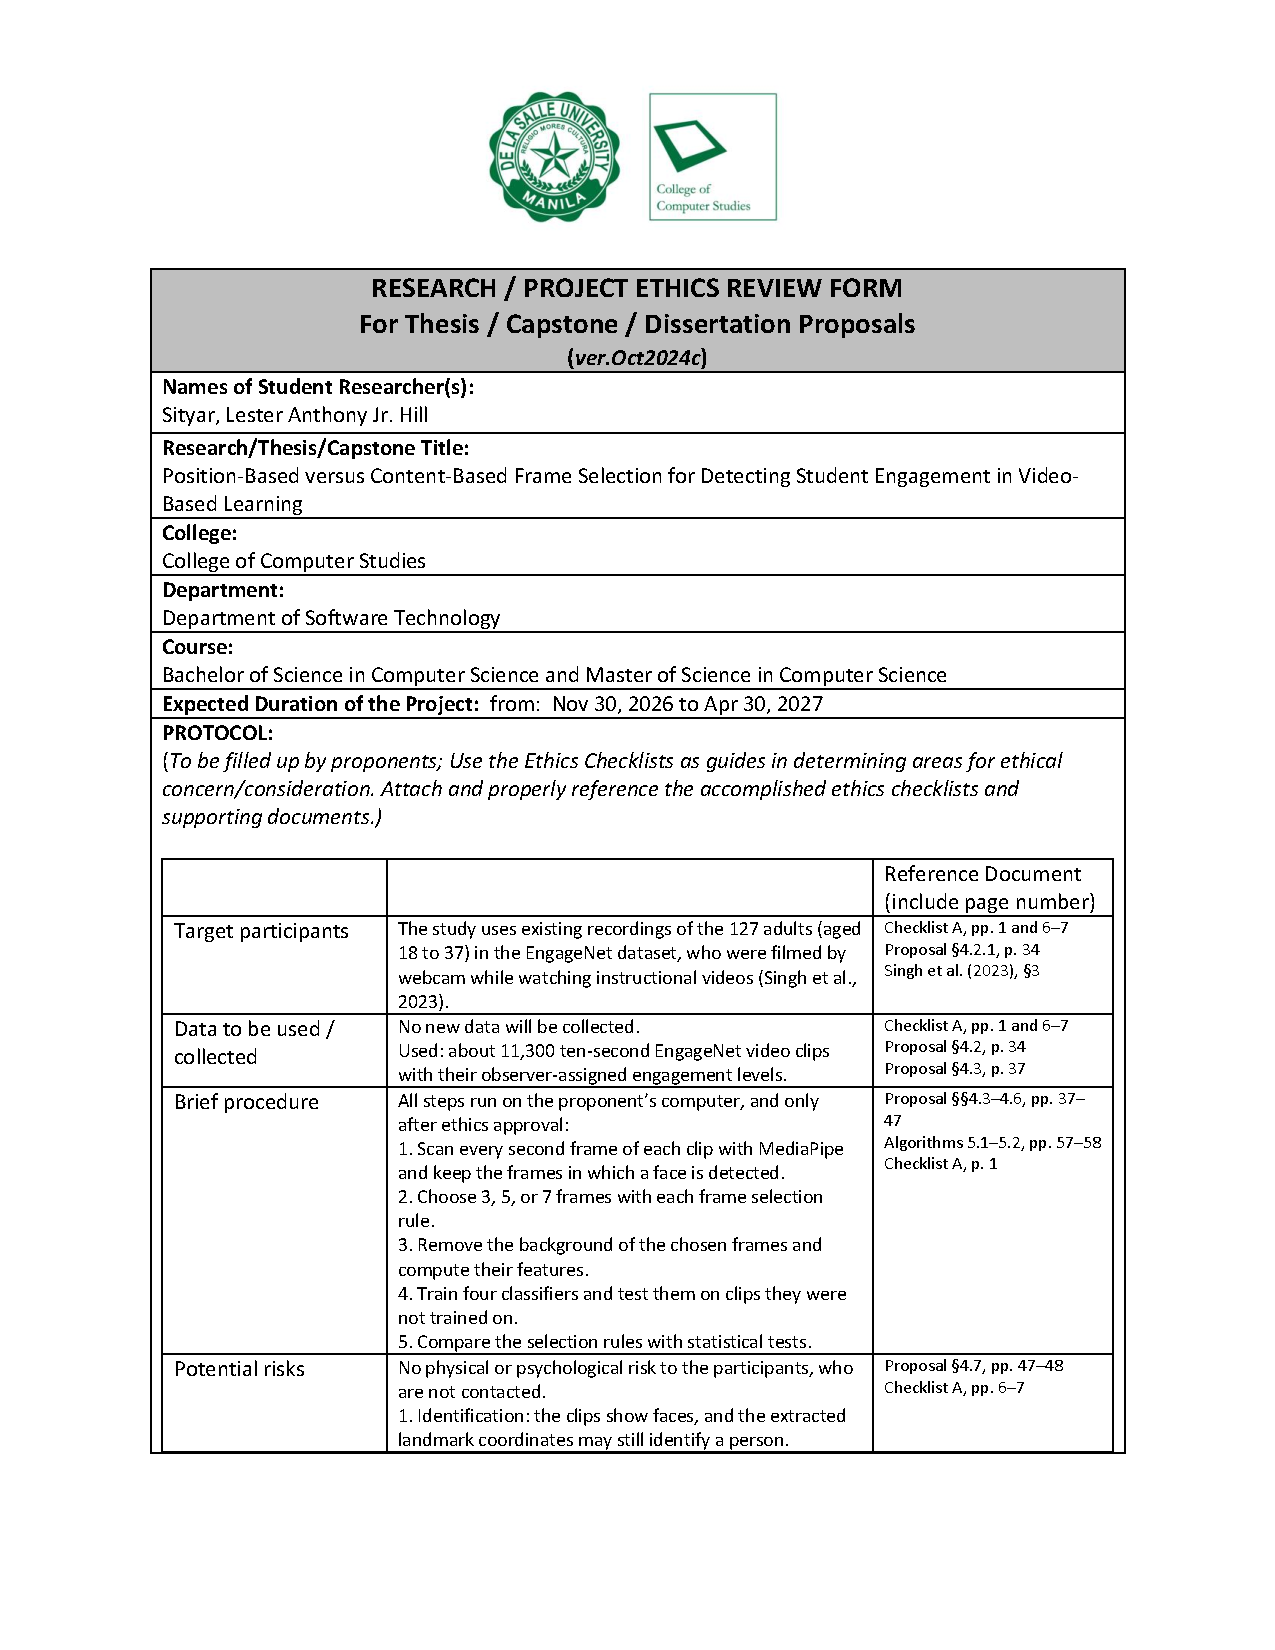
\includepdf[pages=-, scale = 0.9, pagecommand={}, offset = -30 0]{ethics-forms/filled/sityar-ethics-review-form.pdf}

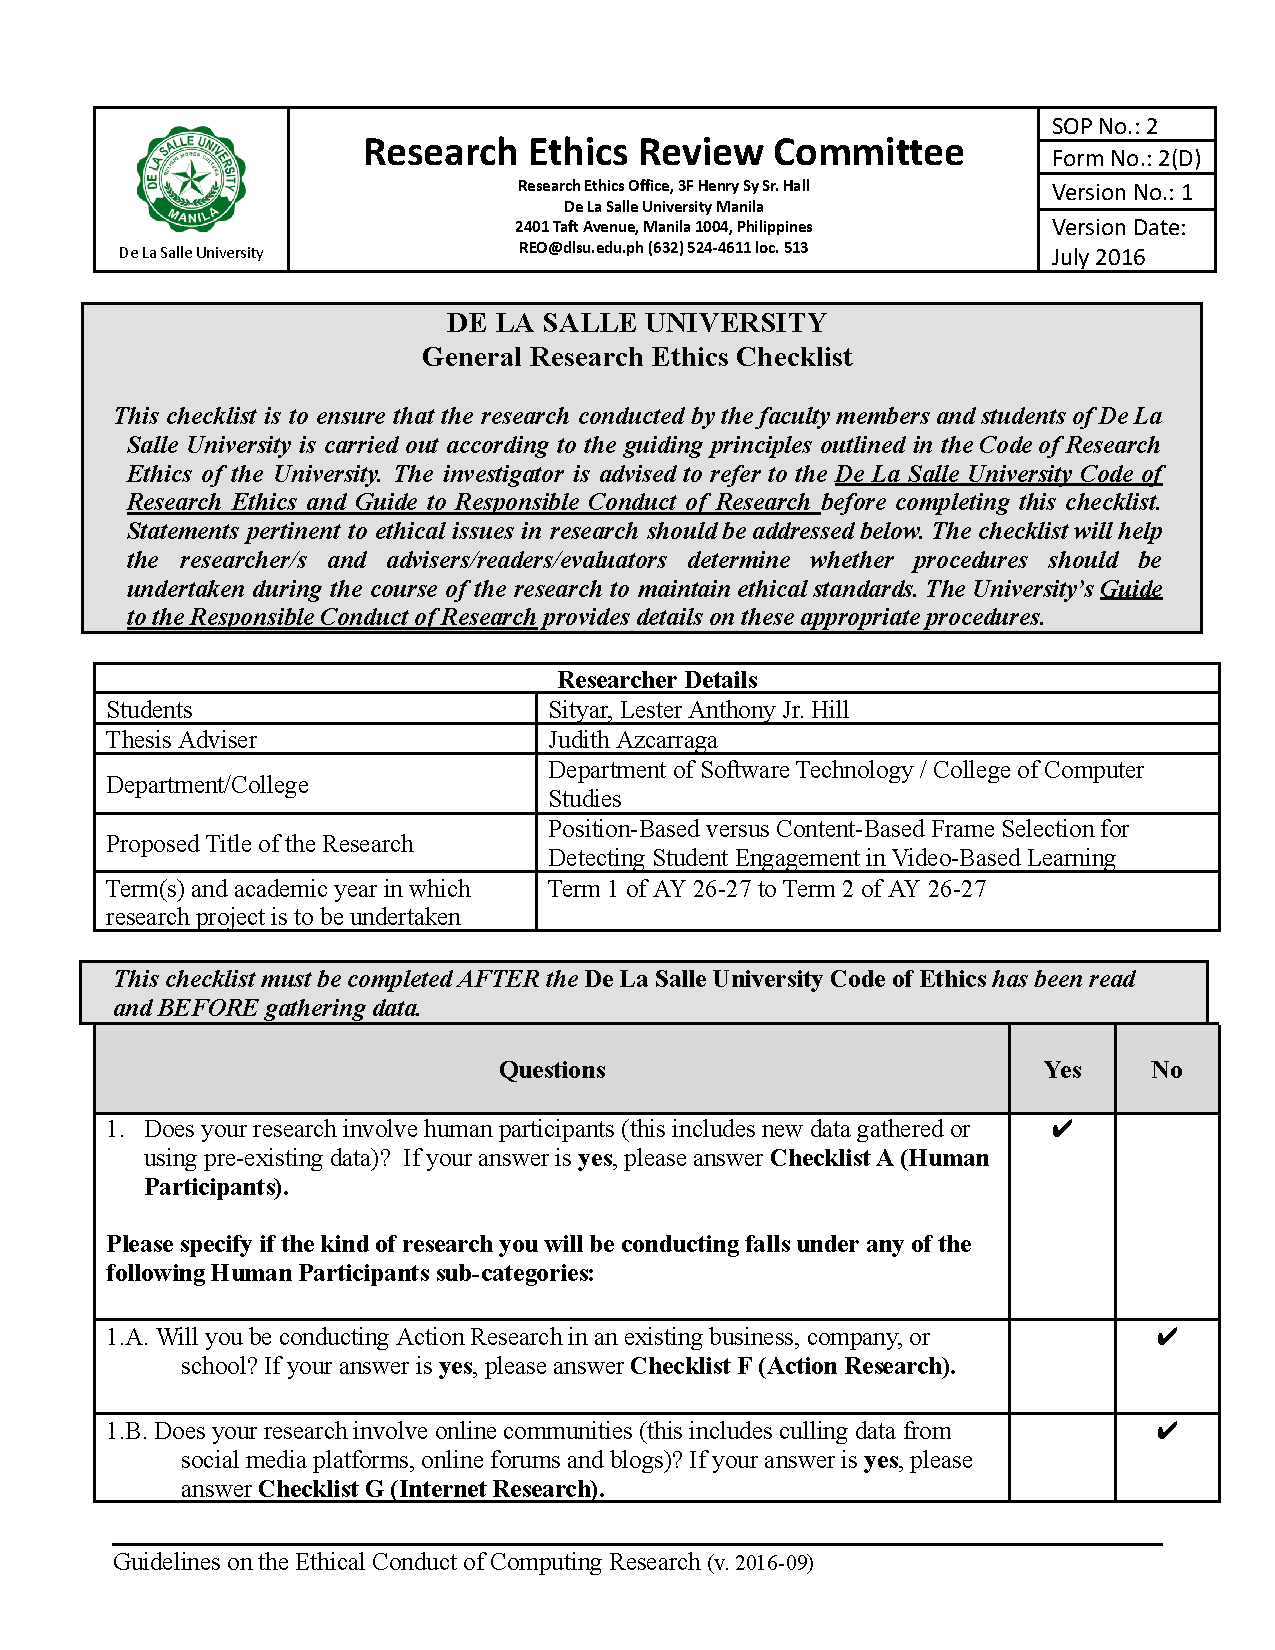
\includepdf[pages=-, scale = 0.9, pagecommand={}, offset = -30 0]{ethics-forms/filled/sityar-general-ethics-checklist.pdf}


\includepdf[pages=-, scale = 0.9, pagecommand={}, offset = -30 0]{ethics-forms/filled/sityar-checklist-a.pdf}

%-- 16 Nov 2026: the signed EngageNet Dataset User Agreement (the approval authority for access named in
%-- Checklist A and the Ethics Review Form), added by the proponent. Same file as docs/EULA_EngageNet_signed.pdf.
%-- Its typed entries (name, institution, date, additional researcher) are FreeText annotations, which pdfpages
%-- drops, so the appendix uses a copy with the annotations flattened into the page (PyMuPDF bake()).
\includepdf[pages=-, scale = 0.9, pagecommand={}, offset = -30 0]{ethics-forms/filled/EULA_EngageNet_signed-flat.pdf}


              %-- includes LaTeX source file for Appendix A
                                  %-- your job: **CREATE/EDIT** your own source file for the appendices
%%%%%%%%%%%%%%%%%%%%%%%%%%%%%%%%%%%%%%%%%%%%%%%%%%%%%%%%%%%%%%%%%%%%%%%%%%%%%%%%%%%%%%%%%%%%%%%%%%%%%%
%
%   Filename    : appendix_publications.tex
%
%   Description : The proponent's three papers, reproduced in full at the adviser's request (15 Nov 2026).
%                 Placed between the ethics documents and the resource persons, so it is Appendix B.
%                 Section 5.1 summarizes the papers in the same order. Statuses are the proponent's
%                 (15 Nov 2026): PERSUASIVE published (LNCS, DOI checked on Crossref); TENCON presented
%                 but not yet published, marked "Accepted for publication" at the proponent's request;
%                 ICCE accepted for presentation. Before the final thesis is deposited online, check the publishers'
%                 rules for reusing the papers (IEEE asks for a credit line and the accepted version).
%
%%%%%%%%%%%%%%%%%%%%%%%%%%%%%%%%%%%%%%%%%%%%%%%%%%%%%%%%%%%%%%%%%%%%%%%%%%%%%%%%%%%%%%%%%%%%%%%%%%%%%%

\chapter{Publications}
\label{sec:publications}

This appendix reproduces the three papers summarized in Section~\ref{sec:prelimwork}, in the order in which they are summarized there. Table~\ref{tab:publications} lists them.

\begin{table}[h]
   \centering
   \caption{Papers reproduced in this appendix}
   \label{tab:publications}
   \small
   \begin{tabular}{llL{2.6cm}c}
      \toprule
      Paper & Venue & Status & Section \\
      \midrule
      \citeA{sityar2026persuasive} & PERSUASIVE 2026 & Published & \ref{sec:daisee} \\
      \citeA{carandang2026tencon} & TENCON 2026 & Accepted for publication & \ref{sec:daisee} \\
      \citeA{sityar2026icce} & ICCE 2026 & Accepted for presentation & \ref{sec:prelim} \\
      \bottomrule
   \end{tabular}
\end{table}

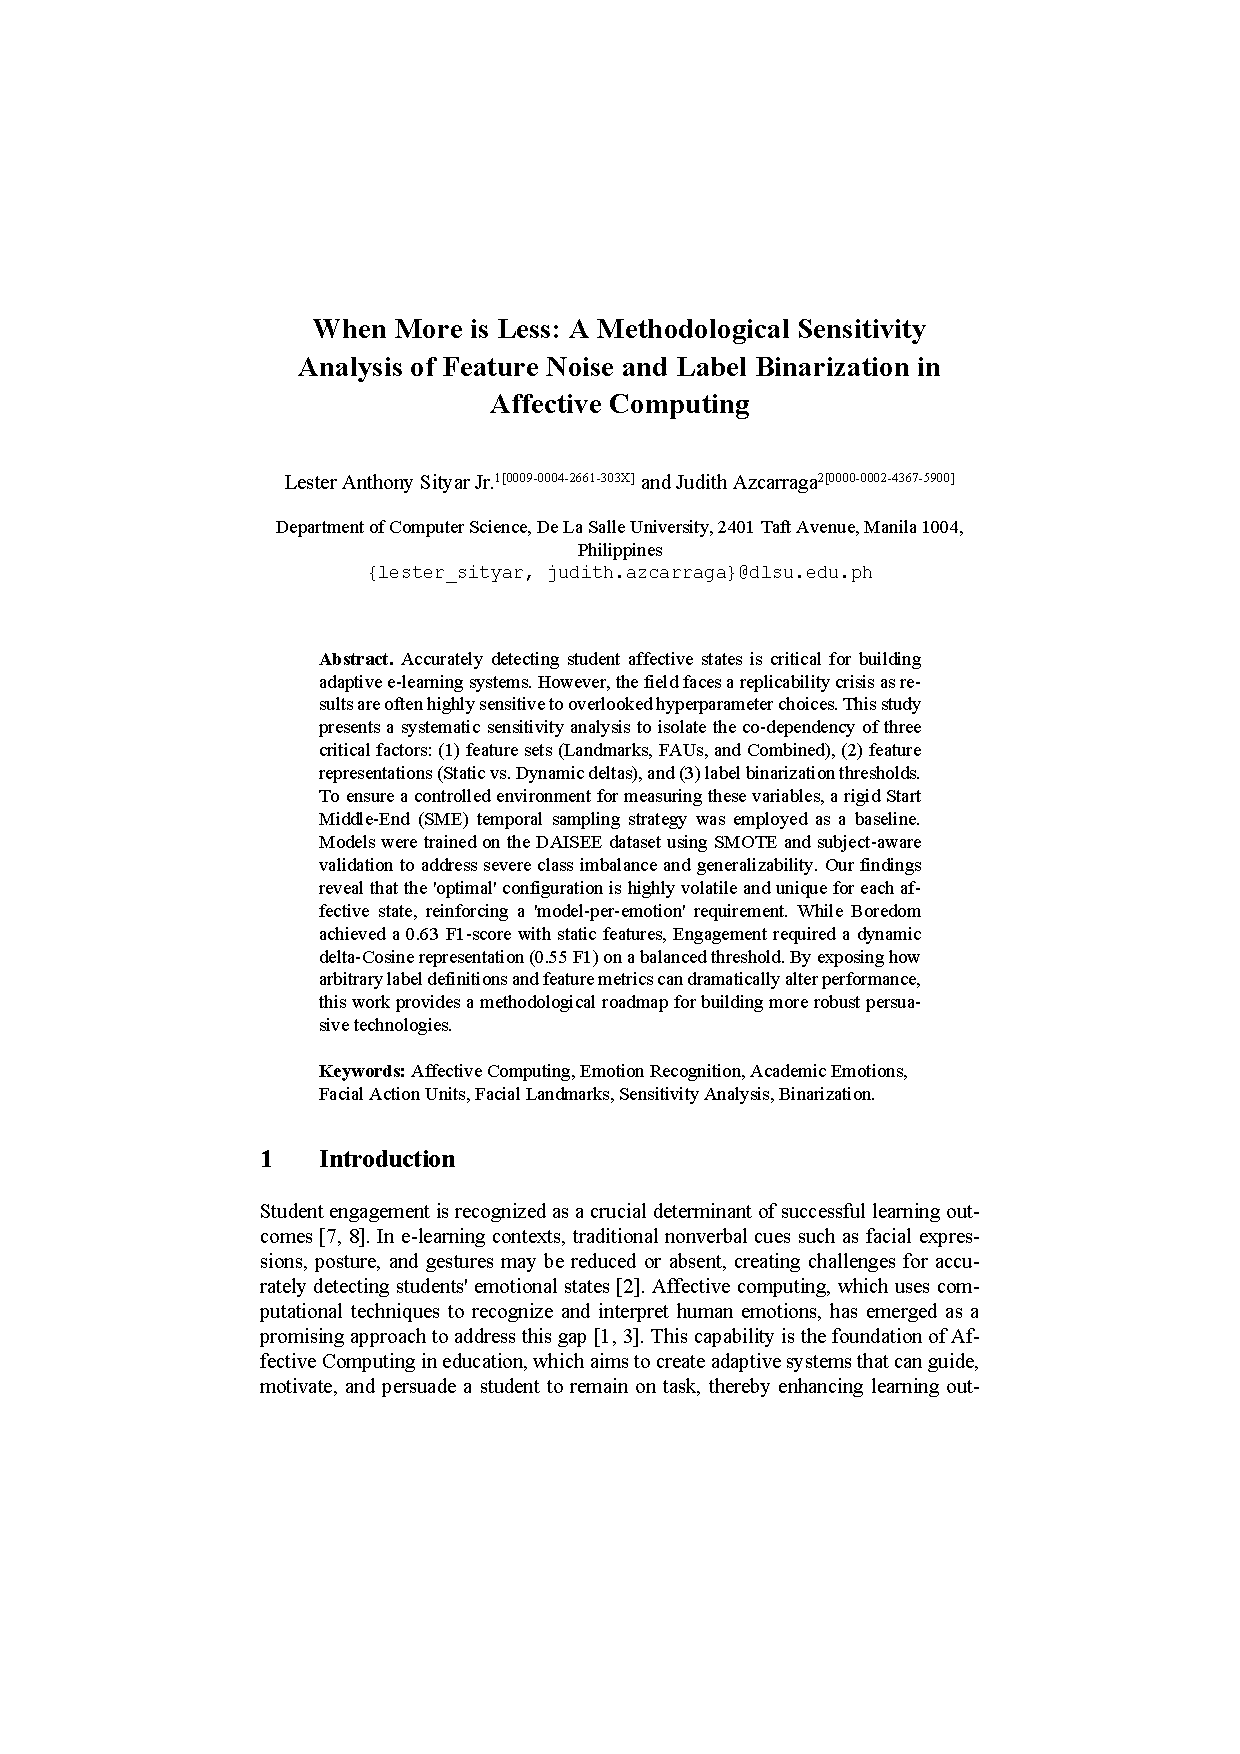
\includepdf[pages=-, scale=0.9, pagecommand={}, offset=-30 0,
   addtotoc={1, section, 1, {When More is Less (PERSUASIVE 2026)}, sec:pub-persuasive}]
   {past-papers/SITYAR-PERSUASIVE2026-Paper.pdf}

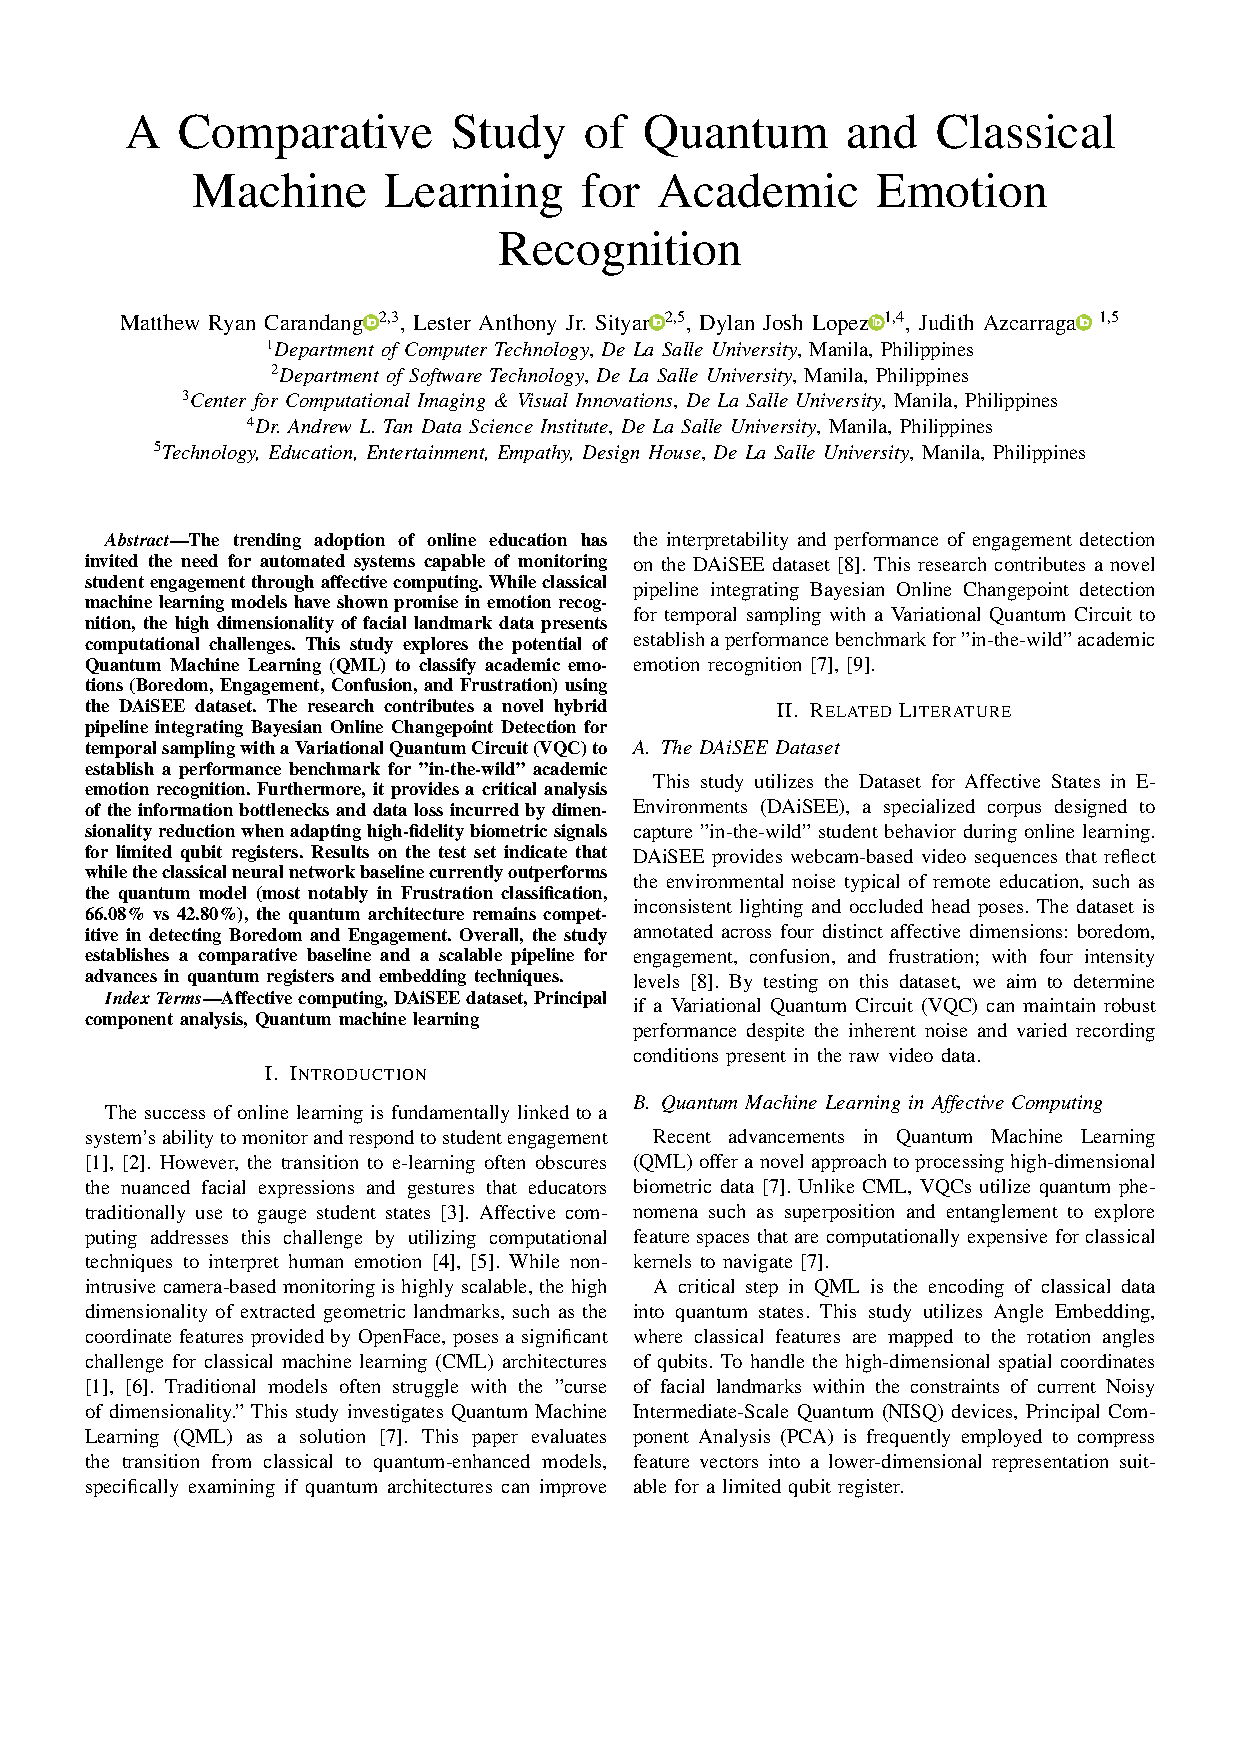
\includepdf[pages=-, scale=0.9, pagecommand={}, offset=-30 0,
   addtotoc={1, section, 1, {A Comparative Study of Quantum and Classical Machine Learning (TENCON 2026)}, sec:pub-tencon}]
   {past-papers/SITYAR-TENCON2026-Paper.pdf}

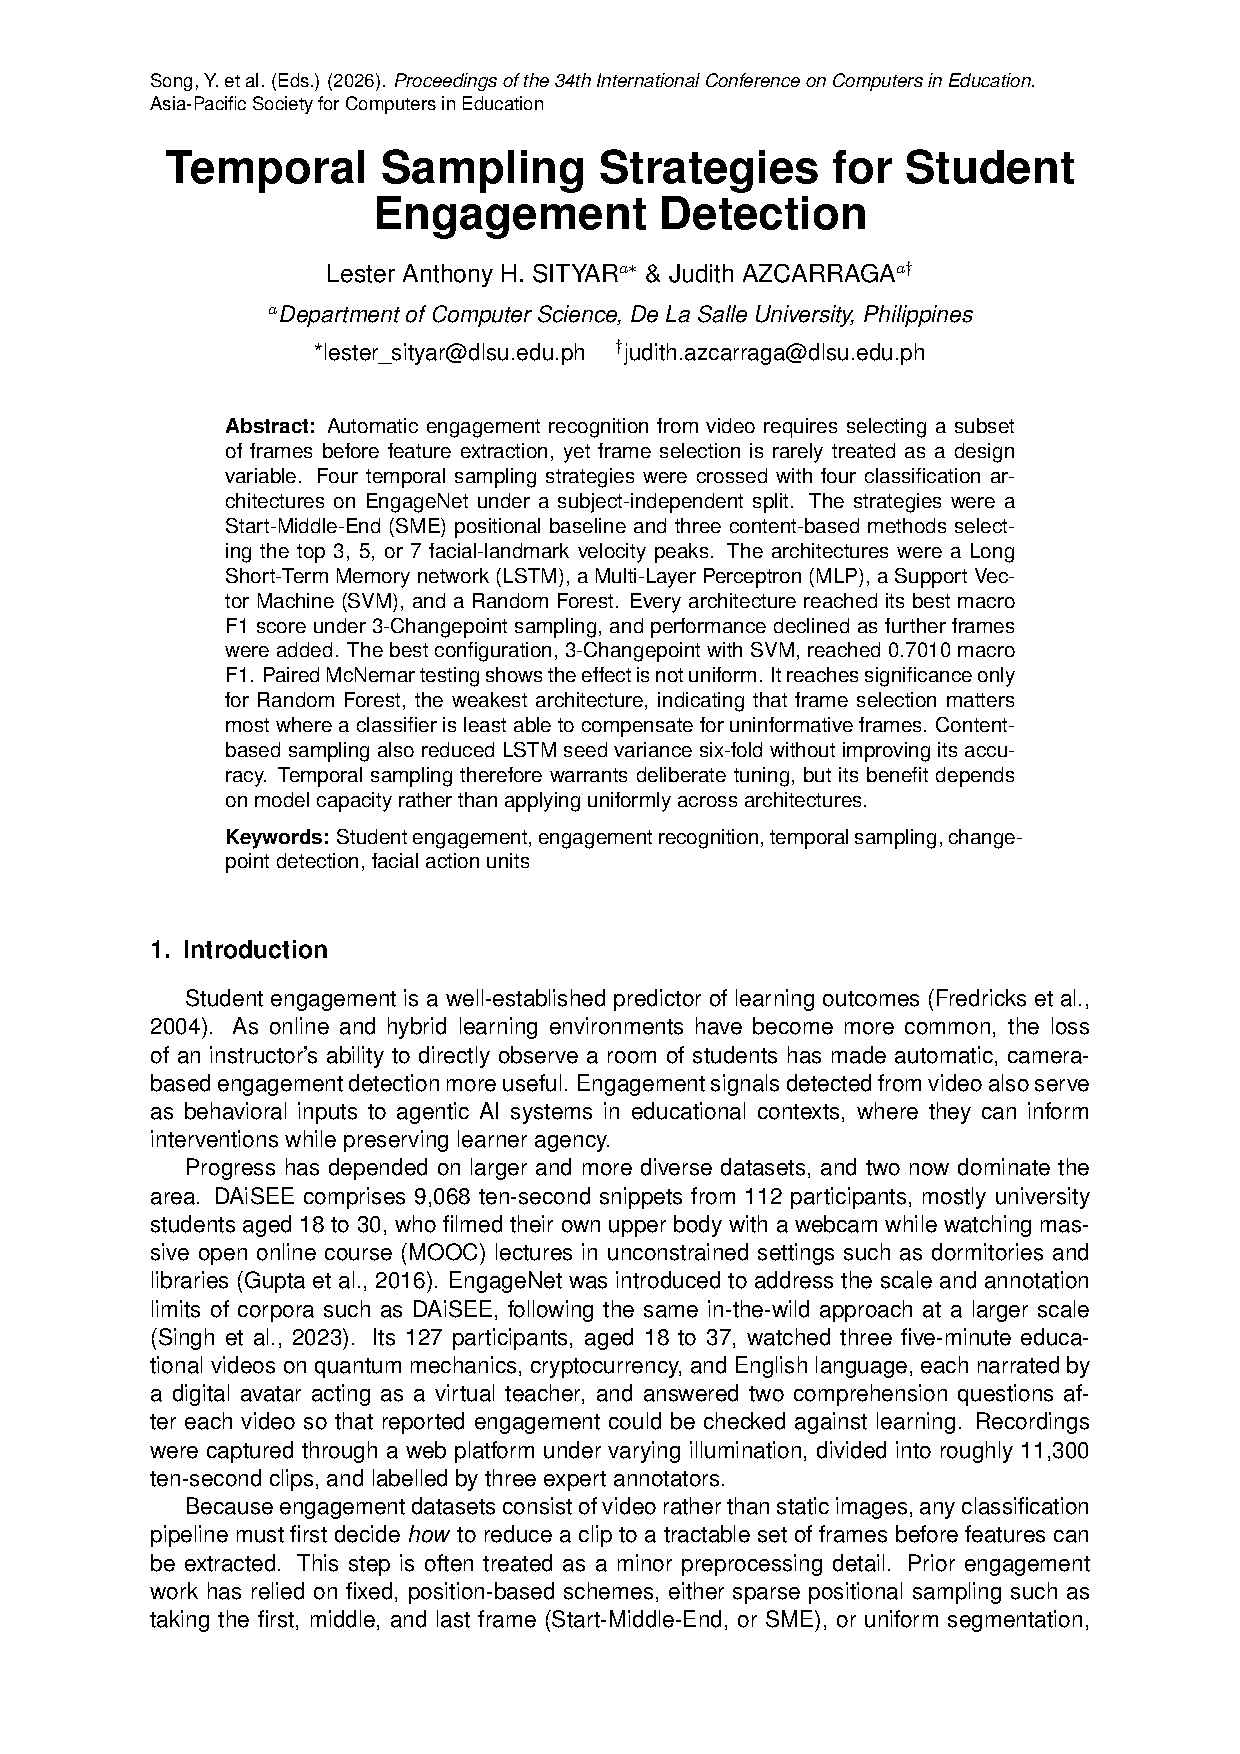
\includepdf[pages=-, scale=0.9, pagecommand={}, offset=-30 0,
   addtotoc={1, section, 1, {Temporal Sampling Strategies for Student Engagement Detection (ICCE 2026)}, sec:pub-icce}]
   {past-papers/SITYAR-ICCE2026-Paper.pdf}
   %-- the proponent's three papers (adviser's request, 15 Nov 2026)
%%%%%%%%%%%%%%%%%%%%%%%%%%%%%%%%%%%%%%%%%%%%%%%%%%%%%%%%%%%%%%%%%%%%%%%%%%%%%%%%%%%%%%%%%%%%%%%%%%%%%%
%
%   Filename    : appendix_B.tex
%
%   Description : This file will contain information about your Resource Persons
%                 
%%%%%%%%%%%%%%%%%%%%%%%%%%%%%%%%%%%%%%%%%%%%%%%%%%%%%%%%%%%%%%%%%%%%%%%%%%%%%%%%%%%%%%%%%%%%%%%%%%%%%%

\chapter{Resource Persons}
\label{sec:appendixc}

%
%  Indicate your resource persons here:
%
%	<full name and title, e.g., Dr. Juan de la Cruz>
%	<profession, e.g., faculty>
%	<department, e.g., College of Computer Studies>
%	<name of institution, e.g., De La Salle University>
%	<e-mail address>
%
%

%
%  the following shows 3 examples, replace entries with your own
%
\newcommand{\resperson}[4]{\textbf{#1} \\ #2 \\ #3 \\ \url{#4}\vspace{0.5em}\\}

%  Add any other resource persons below, in the same five-line form.
\textbf{Dr. Judith J. Azcarraga} \\ Adviser \\ College of Computer Studies\\De La Salle University-Manila \\ \url{judith.azcarraga@dlsu.edu.ph}\vspace{0.5em}\\

              %-- Resource Persons (now Appendix C)


%\bibliographystyle{apacite}       %-- specified APA style for bibliograpy
                                  %-- more details about APA style citation can be found in www.ctan.org/tex-archive/biblio/bibtex/contrib/apacite/

                                  %-- bibliographic entries are handled via bibtex; refer to www.bibtex.org for more details


\bibliography{myreferences}       %-- the file "myreferences.bib" is a sample bibliography (bib) from SIGGRAPH 
                                  %-- your job: **CREATE/EDIT** your own bibliography file  

\end{document}